%%%%%%%%%%%%%%%%%%%%%%%%%%%%%%%%%%%%%%%%%%%%%%%%%%%%%%
\begin{frame}[c]{ }
	\frametitle{Core Hadoop Concepts }
	\centering     
	
	\textcolor{offgreen}{ \large Hadoop Core Components}
\end{frame}
%%%%%%%%%%%%%%%%%%%%%%%%%%%%%%%%%%%%%%%%%%%%%%%%%%%%%%
\begin{frame}[c]{ }
	\frametitle{Data Center Components }
	\begin{figure}
		\centering
		


\tikzset{every picture/.style={line width=0.75pt}} %set default line width to 0.75pt        

\begin{tikzpicture}[x=0.75pt,y=0.75pt,yscale=-1,xscale=1]
	%uncomment if require: \path (0,300); %set diagram left start at 0, and has height of 300
	
	%Shape: Rectangle [id:dp48918224033703217] 
	\draw   (33,20) -- (600,20) -- (600,250) -- (33,250) -- cycle ;
	%Shape: Rectangle [id:dp165115113681796] 
	\draw   (150,40) -- (150,200) -- (50,200) -- (50,40) -- cycle ;
	%Shape: Rectangle [id:dp571567564721695] 
	\draw   (280,40) -- (280,200) -- (180,200) -- (180,40) -- cycle ;
	%Shape: Rectangle [id:dp6858294917527059] 
	\draw   (410,40) -- (410,200) -- (310,200) -- (310,40) -- cycle ;
	%Shape: Rectangle [id:dp026686803204176823] 
	\draw   (540,40) -- (540,200) -- (440,200) -- (440,40) -- cycle ;
	
	%Straight Lines [id:da3697838459968448] 
	\draw    (100,230) -- (490,230) ;
	%Straight Lines [id:da7952384044138053] 
	\draw  [{Circle}-{Circle[open]}] (100,231) -- (100,200) ;
	%Straight Lines [id:da6419250185576916] 
	\draw   [{Circle}-{Circle[open]}]  (230,231) -- (230,200) ;
	%Straight Lines [id:da7501600393941193] 
	\draw   [{Circle}-{Circle[open]}]  (360,231) -- (360,200) ;
	%Straight Lines [id:da9542370953289699] 
	\draw   [{Circle}-{Circle[open]}]  (490,231) -- (490,200) ;
	
	
	

	% Text Node
	\draw (33,3)   node [anchor=north west][inner sep=0.75pt]   [align=left] {{\small Data Center CAI-1234}};
	% Text Node

	\node at (50,26) (rac1)  [anchor=north west][inner sep=0.75pt]  [font=\footnotesize] [align=left] {RAC-A-123};
	% Text Node
	\node at (180,26) (rac2)  [anchor=north west][inner sep=0.75pt]  [font=\footnotesize] [align=left] {RAC-A-456};
	% Text Node
	\node at (310,26) (rac3)  [anchor=north west][inner sep=0.75pt]  [font=\footnotesize] [align=left] {RAC-B-123};
	% Text Node
	\node at (440,26) (rac4)  [anchor=north west][inner sep=0.75pt]  [font=\footnotesize] [align=left] {RAC-B-456};
	
	%rac 1
	\node  [below=of rac1,yshift=1cm,xshift=.4cm]  [scale=.4] (server1){\usebox\Server};
	\node [below=of server1,yshift=1.2cm]  [font=\scriptsize] (server1Lb) {Server 1};

	\node  [below=of server1Lb,yshift=1cm]  [scale=.4] (server2){\usebox\Server};
	\node [below=of server2,yshift=1.2cm]  [font=\scriptsize] (server2Lb) {Server 2};	
	
	%%%rac 2
	\node  [below=of rac2,yshift=1cm,xshift=.4cm]  [scale=.4] (server21){\usebox\Server};
	\node [below=of server21,yshift=1.2cm]  [font=\scriptsize] (server21Lb) {Server 1};
	
	\node  [below=of server21Lb,yshift=1cm]  [scale=.4] (server22){\usebox\Server};
	\node [below=of server22,yshift=1.2cm]  [font=\scriptsize] (server22Lb) {Server 2};	

	%%%rac 3
	\node  [below=of rac3,yshift=1cm,xshift=.4cm]  [scale=.4] (server31){\usebox\Server};
	\node [below=of server31,yshift=1.2cm]  [font=\scriptsize] (server31Lb) {Server 1};
	
	\node  [below=of server31Lb,yshift=1cm]  [scale=.4] (server32){\usebox\Server};
	\node [below=of server32,yshift=1.2cm]  [font=\scriptsize] (server32Lb) {Server 2};	

	%%%rac 4
	\node  [below=of rac4,yshift=1cm,xshift=.4cm]  [scale=.4] (server41){\usebox\Server};
	\node [below=of server41,yshift=1.2cm]  [font=\scriptsize] (server41Lb) {Server 1};
	
	\node  [below=of server41Lb,yshift=1cm]  [scale=.4] (server42){\usebox\Server};
	\node [below=of server42,yshift=1.2cm]  [font=\scriptsize] (server42Lb) {Server 2};	
		
\end{tikzpicture}


	\end{figure}
\end{frame}
%%%%%%%%%%%%%%%%%%%%%%%%%%%%%%%%%%%%%%%%%%%%%%%%%%%%%%
\begin{frame}[c]{ }
	\frametitle{Hadoop Core Concepts }
	
	
	\begin{itemize}  [<+->]
		\item [--] HDFS.
		\item [--] Map-Reduce.
		\item [--] YARN.
		
	\end{itemize}
\end{frame}
%%%%%%%%%%%%%%%%%%%%%%%%%%%%%%%%%%%%%%%%%%%%%%%%%%%%%%
\begin{frame}[c]{ }
	\frametitle{YARN }
	
	\begin{itemize}  [<+->]
		\item [--] YARN =  Yet Another Resource Negotiator.
		\item [--] YARN is responsible for the data-computation framework in Hadoop.
		\item [--] The fundamental idea of YARN is to split up the functionalities of 	\textcolor{offyellow}{ \underline{ \textbf{resource management}}} and 	\textcolor{offyellow}{ \underline{ \textbf{job scheduling/monitoring}}} into separate daemons.
		\item [--] The idea is to have a \textcolor{offyellow}{ \underline{ \textbf{global ResourceManager (RM)}}} and 	\textcolor{offyellow}{ \underline{ \textbf{per-application ApplicationMaster (AM)}}}. 
		\item [--] An application is either a single job or a DAG of jobs.		
	\end{itemize}
			\footnotetext[1]{Apache Hadoop YARN \href{https://hadoop.apache.org/docs/current/hadoop-yarn/hadoop-yarn-site/YARN.html}{https://hadoop.apache.org/docs/current/hadoop-yarn/hadoop-yarn-site/YARN.html}	} 
\end{frame}
%%%%%%%%%%%%%%%%%%%%%%%%%%%%%%%%%%%%%%%%%%%%%%%%%%%%%%
\begin{frame}[c]{ }
	\frametitle{YARN }
	YARN allows to run multiple processing engine on the Hadoop cluster .
	{\footnotesize
	\begin{itemize}  [<+->]
		\item [--] Map-Reduce, Hive, and PIG.
		\item [--] Spark batch, streaming, ML, and SQL.
		\item [--] Impala, Mahoot, and other engines.
	\end{itemize}
	}
\end{frame}
%%%%%%%%%%%%%%%%%%%%%%%%%%%%%%%%%%%%%%%%%%%%%%%%%%%%%%
\begin{frame}[c]{ }
	\frametitle{YARN }

	{\footnotesize
		\begin{itemize}  [<+->]
			\item [--] YARN provides APIs for requesting and working with cluster resources.
			\item [--] These APIs are  not  typically  used  directly  by  user  code.
			\item [--] Users  write  to  higher-level APIs provided by distributed computing frameworks, Ex: (Map-reduce or Spark on yarn), which themselves are built on YARN and hide the resource management details from the user..
		\end{itemize}
	}
			\footnotetext[1]{Hadoop the defenitive guide Ch.4 P.79. \href{https://hadoop.apache.org/docs/current/hadoop-yarn/hadoop-yarn-site/YARN.html}{https://hadoop.apache.org/docs/current/hadoop-yarn/hadoop-yarn-site/YARN.html}} 
			\footnotetext[1]{Apache Hadoop YARN Ch.4 P.43. \href{https://www.oreilly.com/library/view/apache-hadooptm-yarn/9780133441925/}{https://www.oreilly.com/library/view/apache-hadooptm-yarn/9780133441925/}} 
\end{frame}
%%%%%%%%%%%%%%%%%%%%%%%%%%%%%%%%%%%%%%%%%%%%%%%%%%%%%%
\begin{frame}[c]{ }
	\frametitle{YARN }
	In YARN, there are at least three actors:	
	{\footnotesize
		\begin{itemize}  [<+->]
			\item The clinet : The Job Submitter.
			\item Node(s) Master: the Resource Manager.
			\item Data Node(s): the Node Manager.
		\end{itemize}
}

\end{frame}
%%%%%%%%%%%%%%%%%%%%%%%%%%%%%%%%%%%%%%%%%%%%%%%%%%%%%%
\begin{frame}[c]{ }
	\frametitle{YARN Components Hierarchy}
	
	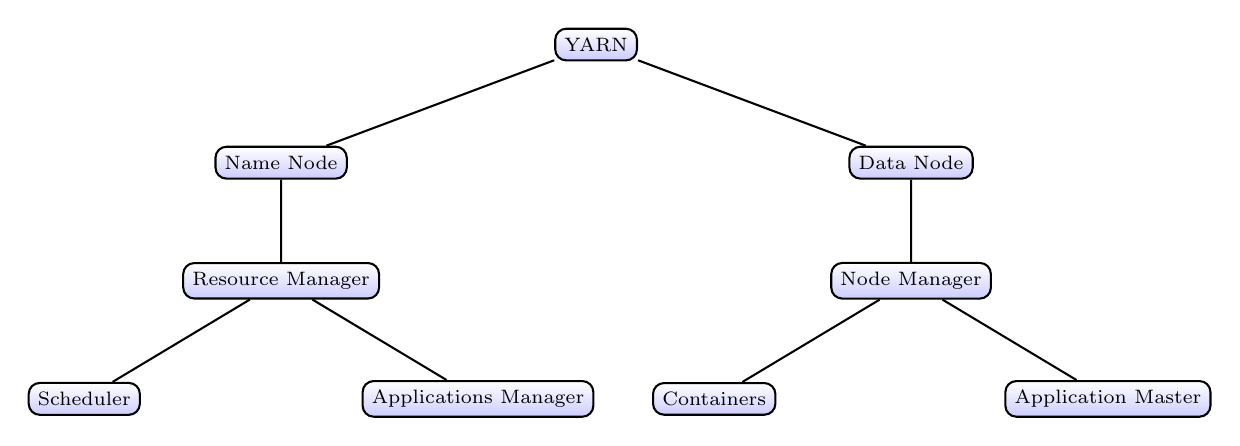
\begin{tikzpicture}[every node/.style={shape=rectangle, rounded corners,
			draw, align=center,
			top color=white, bottom color=blue!20,font=\scriptsize,color=black},level 1/.style={sibling distance=80mm},level 2/.style={sibling distance=50mm}
		]
		\node {YARN}
		child { node {Name Node} 
			child { node {Resource Manager} child { node {Scheduler} }  child { node {Applications Manager}}}
		}
		child { node {Data Node}  child {node {Node Manager} child {node {Containers}} child {node {Application Master}}}}
		;
	\end{tikzpicture}
	
\end{frame}
%%%%%%%%%%%%%%%%%%%%%%%%%%%%%%%%%%%%%%%%%%%%%%%%%%%%%%
\begin{frame}[c]{ }
	\frametitle{YARN Daemon}
	YARN (The data-computation framework) consists of
		\begin{itemize}  [<+->]
			\item [--] Resource Manager (long-running daemon): It is \textcolor{offyellow}{ \underline{ \textbf{one per cluster}}} to manage the use of resources across the cluster.
			\item [--] Node Manager: It is running on all the nodes in the cluster to launch and monitor \textcolor{offyellow}{ \underline{ \textbf{containers}}}
		\end{itemize}

\end{frame}

%%%%%%%%%%%%%%%%%%%%%%%%%%%%%%%%%%%%%%%%%%%%%%%%%%%%%%
\begin{frame}[c]{ }
	\frametitle{Resource Manager }
	The Resource Manager has two main components
	{\footnotesize
		\begin{itemize}  [<+->]
			\item [--] Scheduler.
			\item [--] Applications Manager.
		\end{itemize}
	}
\end{frame}
%%%%%%%%%%%%%%%%%%%%%%%%%%%%%%%%%%%%%%%%%%%%%%%%%%%%%%
\begin{frame}[c]{ }
	\frametitle{Resource Manager }
	{\footnotesize
		\begin{itemize}  [<+->]
			\item [--] It runs on the master node.
			\item [--] It is the ultimate authority that arbitrates resources among all the applications in the system.
			\item [--] It is the global resource schedule.
			\item [--] It is a single point of failure in YARN. We can acheive HA with an active-standby configuration.
		\end{itemize}
	}
\end{frame}
%%%%%%%%%%%%%%%%%%%%%%%%%%%%%%%%%%%%%%%%%%%%%%%%%%%%%%
\begin{frame}[c]{ }
	\frametitle{Resource Manager - Applications Manager}
	
	{\footnotesize
		\begin{itemize}  [<+->]
			\item [--] It is responsible for accepting job submissions.
			\item [--] It is responsible for negotiating the first container for executing the application specific \textcolor{offyellow}{ \underline{ \textbf{ApplicationMaster}}}.
			\item [--] After application submission
			\begin{itemize}  [<+-> \color{almond}]
				\item It first validates the application’s specifications.
				\item It rejects any application that requests unsatisfiable resources for its ApplicationMaster (i.e., no node in the cluster has enough resources to run the ApplicationMaster itself).
				\item It then ensures that no other application was already submitted with the same application ID.
				\item It forwards the admitted application to the scheduler.
			\end{itemize}
		\end{itemize}
	}
\end{frame}
%%%%%%%%%%%%%%%%%%%%%%%%%%%%%%%%%%%%%%%%%%%%%%%%%%%%%%
\begin{frame}[c]{ }
	\frametitle{Resource Manager - Applications Manager}
	
	{\footnotesize
		\begin{itemize}  [<+->]
			\item [--] It is responsible for recording and managing finished applications for a while before being completely evacuated from the ResourceManager’s memory.
			\item [--] It places an ApplicationSummary in the daemon’s log file after the application finishes.
			\item [--] Finally, the ApplicationsManager keeps a cache of completed applications long after applications finish to support users’ requests for application data
		\end{itemize}
	}
	
\end{frame}
%%%%%%%%%%%%%%%%%%%%%%%%%%%%%%%%%%%%%%%%%%%%%%%%%%%%%%
\begin{frame}[c]{ }
	\frametitle{Resource Manager -  Scheduler}	
	{\footnotesize
		\begin{itemize}  [<+->]
			\item [--] It is responsible for allocating resources to the various running applications subject to familiar constraints of capacities, queues etc.
			\item [--] It performs its scheduling function based on the resource requirements of the applications.
			\item [--] It does so based on the abstract notion of a resource \textcolor{offyellow}{ \underline{ \textbf{containers}}} which incorporates elements such as memory, cpu, disk, network etc.
			\item [--] The current schedulers such as the \textcolor{offyellow}{ \underline{ \textbf{CapacityScheduler}}} and the \textcolor{offyellow}{ \underline{ \textbf{FairScheduler}}} would be some examples of plug-ins.
		\end{itemize}
	}
\end{frame}

%%%%%%%%%%%%%%%%%%%%%%%%%%%%%%%%%%%%%%%%%%%%%%%%%%%%%%
\begin{frame}[c]{ }
	\frametitle{Node Manager }
		The Node Manager has two main components
		\begin{itemize}  [<+->]
			\item [--] Containers
			\item [--] Application Master (AM)
		\end{itemize}
\end{frame}
%%%%%%%%%%%%%%%%%%%%%%%%%%%%%%%%%%%%%%%%%%%%%%%%%%%%%%
\begin{frame}[c]{ }
	\frametitle{Node Manager }
	{\footnotesize
		\begin{itemize}  [<+->]
			\item [--] It runs on the data node.
			\item [--] It is YARN’s per-node “worker” agent, taking care of the individual compute nodes in a Hadoop cluster.
			\item [--] On start-up, the NodeManager registers with the ResourceManager; it then sends heartbeats with its status and waits for instructions. 
			\item [--] Its primary goal is to manage application containers assigned to it by the ResourceManager.
		\end{itemize}
	}
\end{frame}
%%%%%%%%%%%%%%%%%%%%%%%%%%%%%%%%%%%%%%%%%%%%%%%%%%%%%%
\begin{frame}[c]{ }
	\frametitle{Node Manager }
	Node Manager is responsilble for 
	{\footnotesize
		\begin{itemize}  [<+->]
			\item [--] Node Status Updater: Keeping up-to-date with the ResourceManage.
			\item [--] Container Manager: Overseeing application containers’ life-cycle management, and monitoring resource usage (memory, CPU) of individual containers.
			\item [--] Node Health Checker Service: Tracking node health.
			\item [--] Log Handler: keeping the containers’ logs, and uploading them onto a file-system.
		\end{itemize}
	}
\end{frame}
%%%%%%%%%%%%%%%%%%%%%%%%%%%%%%%%%%%%%%%%%%%%%%%%%%%%%%
\begin{frame}[c]{ }
	\frametitle{Node Manager - Containers }
	
	{\footnotesize
		\begin{itemize}  [<+->]
			\item [--] A container is a collection of physical resources such as RAM, CPU cores, and disks on a single node.
			\item [--] There can be multiple containers on a single node.
			\item [--] Every node in the system is considered to be composed of multiple containers of minimum size of memory (e.g., 512 MB or 1 GB) and CPU.
			\item [--] A container executes an application-specific process with a constrained set of resources(memory, CPU, and so on).
			\item [--] RM is creating containers based on the application requirements. 
			\item [--] ApplicaIons run in one or more containers.
			\item [--] A container is supervised by the NodeManager and scheduled by the ResourceManager.
		\end{itemize}
	}
\end{frame}
%%%%%%%%%%%%%%%%%%%%%%%%%%%%%%%%%%%%%%%%%%%%%%%%%%%%%%
\begin{frame}[c]{ }
	\frametitle{Node Manager - Containers }
	
	{\footnotesize
		\begin{itemize}  [<+->]
			\item [--] Each application starts out as an ApplicationMaster, which is itself a container (often referred to as container 0).
			\item [--] Once started, the ApplicationMaster must negotiate with the ResourceManager for more containers.
			\item [--] Container requests (and releases) can take place in a dynamic fashion at run time. For instance, a MapReduce job may request a certain amount of mapper containers; as they finish their tasks, it may release them and request more reducer containers to be started.
		\end{itemize}
	}
\end{frame}
%%%%%%%%%%%%%%%%%%%%%%%%%%%%%%%%%%%%%%%%%%%%%%%%%%%%%%
\begin{frame}[c]{ }
	\frametitle{Node Manager - Application Master }
	
	{\footnotesize
		\begin{itemize}  [<+->]
			\item [--] The ApplicationMaster is the process that coordinates an application’s execution in the cluster (It runs in container 0).

			\item [--] Each application has its own unique ApplicationMaster (one per applicaIon), which is tasked with negotiating resources (containers) from the ResourceManager and working with the NodeManager(s) to execute and monitor the tasks.

			\item [--] It will periodically send heartbeats to the ResourceManager to affirm its health and to update the record of its resource demands.

			\item [--] It is framework/applicaIon specific.			

		\end{itemize}
	}
\end{frame}

%%%%%%%%%%%%%%%%%%%%%%%%%%%%%%%%%%%%%%%%%%%%%%%%%%%%%%
\begin{frame}[c]{ }
	\frametitle{Running an Application on YARN - Submit Application}
	\begin{figure}
		\centering
		\tikzset{every picture/.style={line width=0.75pt}} %set default line width to 0.75pt        

\begin{tikzpicture}[x=0.75pt,y=0.75pt,yscale=-1,xscale=1]
		
	
	% Text Node
	\node (11,3.17) (com) [anchor=north west][inner sep=0.75pt]  [font=\scriptsize] [align=left] {$\displaystyle \$\ \ $ \textcolor{offgreen}{hadoop} \textcolor{white}{ jar my-app.jar} \textcolor{offyellow}{sales\_data}};
	
	%uncomment if require: \path (0,300); %set diagram left start at 0, and has height of 300
	\node  [below=of com,yshift=1cm,xshift=-.3cm]  [scale=.4] (clientPC){\usebox\Server};
	\node [below=of clientPC,yshift=1.2cm]  [font=\footnotesize] (clientLb) {client};
	
	%Shape: Rectangle [id:dp5619170157619483] 
	\draw   (7.23,120) -- (115,120) -- (115,178) -- (7.23,178) -- cycle ;
	\node  at (90,150) [scale=.4] (clientPC){\usebox\Server};
	%Straight Lines [id:da31002175643328755] 
	\draw [->]   (78,90) -- (79.05,118) ;
	
	%%%data node boxes
	%Shape: Rectangle [id:dp554125548261542] 
	\draw   (223,10) -- (418,10) -- (418,51.17) -- (223,51.17) -- cycle ;
	\node  at (400,30) [scale=.3] (datanode){\usebox\Server};
	%Shape: Rectangle [id:dp9273881082754108] 
	\draw   (223,69) -- (418,69) -- (418,110.17) -- (223,110.17) -- cycle ;
	\node  at (400,89) [scale=.3] (datanode){\usebox\Server};
	%Shape: Rectangle [id:dp8796814929656595] 
	\draw   (223,129) -- (418,129) -- (418,170.17) -- (223,170.17) -- cycle ;
	\node  at (400,149) [scale=.3] (datanode){\usebox\Server};
	%Shape: Rectangle [id:dp17827363758413817] 
	\draw   (223,186) -- (418,186) -- (418, 227.17) -- (223,227.17) -- cycle ;
	\node  at (400,206) [scale=.3] (datanode){\usebox\Server};
	\draw (350,230) node [anchor=north west][inner sep=0.75pt]  [font=\footnotesize] [align=left] {Data Nodes};
	
	
	%%%long line
	%Straight Lines [id:da14914786071792174] 
	\draw    (202,21) -- (202,208) ;
	%Straight Lines [id:da8867292837129914] 
	\draw    (202,21) -- (221,21) ;
	%Straight Lines [id:da5461355192839608] 
	\draw    (202,90) -- (221,90) ;
	%Straight Lines [id:da062355905035047066] 
	\draw    (202,148) -- (221,148) ;
	%Straight Lines [id:da003049579272986991] 
	\draw    (202,208) -- (221,208) ;
	
	%%%Node Manager
	\draw  [color={rgb, 255:red, 0; green, 0; blue, 0 }  ,draw opacity=1 ][fill={rgb, 255:red, 126; green, 211; blue, 33 }  ,fill opacity=1 ] (225,12) -- (300.1,12) -- (300.1,28.17) -- (225,28.17) -- cycle ;
	\draw  [color={rgb, 255:red, 0; green, 0; blue, 0 }  ,draw opacity=1 ][fill={rgb, 255:red, 126; green, 211; blue, 334 }  ,fill opacity=1 ] (225,71) -- (300.1,71) -- (300.1,87.17) -- (225,87.17) -- cycle ;
	\draw  [color={rgb, 255:red, 0; green, 0; blue, 0 }  ,draw opacity=1 ][fill={rgb, 255:red, 126; green, 211; blue, 33 }  ,fill opacity=1 ] (225,131) -- (300.1,131) -- (300.1,148.17) -- (225,148.17) -- cycle ;
	\draw  [color={rgb, 255:red, 0; green, 0; blue, 0 }  ,draw opacity=1 ][fill={rgb, 255:red, 126; green, 211; blue, 33 }  ,fill opacity=1 ] (225,188) -- (300.1,188) -- (300.1,205.17) -- (225,205.17) -- cycle ;
	
	
	%%%% Name Node
	\draw   (482,115) -- (588,115) -- (588,183) -- (482,183) -- cycle ;
	\node  at (563,150) [scale=.5] (clientPC){\usebox\Server};
	\draw (486,141) node [anchor=north west][inner sep=0.75pt]  [font=\footnotesize] [align=left] {Name \\Node};

	
	\draw (13,141) node [anchor=north west][inner sep=0.75pt]  [font=\footnotesize] [align=left] {Resource \\Manager};
	
	
	
	% Text Node
	\draw (225,13) node [anchor=north west][inner sep=0.75pt]  [font=\scriptsize,color=black] [align=left] {Node Manager};	
	\draw (225,72) node [anchor=north west][inner sep=0.75pt]  [font=\scriptsize,color=black] [align=left] {Node Manager};
	\draw (225,132) node [anchor=north west][inner sep=0.75pt]  [font=\scriptsize,color=black] [align=left] {Node Manager};
	\draw (225,189) node [anchor=north west][inner sep=0.75pt]  [font=\scriptsize,color=black] [align=left] {Node Manager};
	
	%circles
	\draw[fill={rgb, 255:red, 74; green, 144; blue, 226 }, thick] (50,95) circle (.2 cm);
	\draw (45,90) node [anchor=north west][inner sep=0.75pt]  [font=\footnotesize] [align=left] {1};
	
	%Blocks
	% Text Node
	\draw[fill={rgb, 255:red, 245; green, 166; blue, 35 }, thick] (310,38) circle (.25cm);
	\draw (303,33) node [anchor=north west][inner sep=0.75pt]  [font=\scriptsize,color=black] [align=left] {B1};
	
	
	% Text Node
	\draw[fill={rgb, 255:red, 245; green, 166; blue, 35 }, thick] (310,97) circle (.25cm);
	\draw (303,92) node [anchor=north west][inner sep=0.75pt]  [font=\scriptsize,color=black] [align=left] {B2};
	
	% Text Node
	\draw[fill={rgb, 255:red, 245; green, 166; blue, 35 }, thick] (310,214) circle (.25cm);
	\draw (303,209) node [anchor=north west][inner sep=0.75pt]  [font=\scriptsize,color=black] [align=left] {B3};
	
 	\draw (465,20) node [draw,rectangle,fill=mauve,text width=3cm,text centered]   [anchor=north west] [inner sep=3pt]  [font=\bfseries,font=\scriptsize] [align=left] { A client submits the app including the specifications to  launch the application-specific AM};
 	
	
\end{tikzpicture}

	\end{figure}
\end{frame}
%%%%%%%%%%%%%%%%%%%%%%%%%%%%%%%%%%%%%%%%%%%%%%%%%%%%%%%
%\begin{frame}[c]{ }
%	\frametitle{Running an Application on Hadoop-YARN }
%	\begin{figure}
%		\centering
%		\tikzset{every picture/.style={line width=0.75pt}} %set default line width to 0.75pt        

\begin{tikzpicture}[x=0.75pt,y=0.75pt,yscale=-1,xscale=1]
	%uncomment if require: \path (0,300); %set diagram left start at 0, and has height of 300
	\node  [below=of com,yshift=1.2cm,xshift=-1.4cm]  [scale=.4] (clientPC){\usebox\Server};
	\node [below=of clientPC,yshift=1.2cm]  [font=\footnotesize] (clientLb) {client};
	
	%Shape: Rectangle [id:dp5619170157619483] 
	\draw   (7.23,120) -- (115,120) -- (115,178) -- (7.23,178) -- cycle ;
	\node  at (90,150) [scale=.4] (clientPC){\usebox\Server};
	%Straight Lines [id:da31002175643328755] 
	\draw [->]   (78,90) -- (79.05,118) ;
	
	%%%data node boxes
	%Shape: Rectangle [id:dp554125548261542] 
	\draw   (223,10) -- (418,10) -- (418,51.17) -- (223,51.17) -- cycle ;
	\node  at (400,30) [scale=.3] (datanode){\usebox\Server};
	%Shape: Rectangle [id:dp9273881082754108] 
	\draw   (223,69) -- (418,69) -- (418,110.17) -- (223,110.17) -- cycle ;
	\node  at (400,89) [scale=.3] (datanode){\usebox\Server};
	%Shape: Rectangle [id:dp8796814929656595] 
	\draw   (223,129) -- (418,129) -- (418,170.17) -- (223,170.17) -- cycle ;
	\node  at (400,149) [scale=.3] (datanode){\usebox\Server};
	%Shape: Rectangle [id:dp17827363758413817] 
	\draw   (223,186) -- (418,186) -- (418, 227.17) -- (223,227.17) -- cycle ;
	\node  at (400,206) [scale=.3] (datanode){\usebox\Server};
	\draw (350,230) node [anchor=north west][inner sep=0.75pt]  [font=\footnotesize] [align=left] {Data Nodes};
	
	
	%%%long line
	%Straight Lines [id:da14914786071792174] 
	\draw    (202,21) -- (202,208) ;
	%Straight Lines [id:da8867292837129914] 
	\draw    (202,21) -- (221,21) ;
	%Straight Lines [id:da5461355192839608] 
	\draw    (202,90) -- (221,90) ;
	%Straight Lines [id:da062355905035047066] 
	\draw    (202,148) -- (221,148) ;
	%Straight Lines [id:da003049579272986991] 
	\draw    (202,208) -- (221,208) ;
	
	%%%Node Manager
	\draw  [color={rgb, 255:red, 0; green, 0; blue, 0 }  ,draw opacity=1 ][fill={rgb, 255:red, 126; green, 211; blue, 33 }  ,fill opacity=1 ] (225,12) -- (300.1,12) -- (300.1,28.17) -- (225,28.17) -- cycle ;
	\draw  [color={rgb, 255:red, 0; green, 0; blue, 0 }  ,draw opacity=1 ][fill={rgb, 255:red, 126; green, 211; blue, 334 }  ,fill opacity=1 ] (225,71) -- (300.1,71) -- (300.1,87.17) -- (225,87.17) -- cycle ;
	\draw  [color={rgb, 255:red, 0; green, 0; blue, 0 }  ,draw opacity=1 ][fill={rgb, 255:red, 126; green, 211; blue, 33 }  ,fill opacity=1 ] (225,131) -- (300.1,131) -- (300.1,148.17) -- (225,148.17) -- cycle ;
	\draw  [color={rgb, 255:red, 0; green, 0; blue, 0 }  ,draw opacity=1 ][fill={rgb, 255:red, 126; green, 211; blue, 33 }  ,fill opacity=1 ] (225,188) -- (300.1,188) -- (300.1,205.17) -- (225,205.17) -- cycle ;
	
	
	%%%% Name Node
	\draw   (482,115) -- (588,115) -- (588,183) -- (482,183) -- cycle ;
	\node  at (563,150) [scale=.5] (clientPC){\usebox\Server};
	\draw (486,141) node [anchor=north west][inner sep=0.75pt]  [font=\footnotesize] [align=left] {Name \\Node};
	
	
	% Text Node
	\node (11,3.17) (com) [anchor=north west][inner sep=0.75pt]  [font=\scriptsize] [align=left] {$\displaystyle \$\ \ $ \textcolor{offgreen}{hadoop} \textcolor{white}{ jar my-app.jar} \textcolor{offyellow}{sales\_data}};
	
	
	\draw (13,141) node [anchor=north west][inner sep=0.75pt]  [font=\footnotesize] [align=left] {Resource \\Manager};

	
	
	% Text Node
	\draw (225,13) node [anchor=north west][inner sep=0.75pt]  [font=\scriptsize,color=black] [align=left] {Node Manager};	
	\draw (225,72) node [anchor=north west][inner sep=0.75pt]  [font=\scriptsize,color=black] [align=left] {Node Manager};
	\draw (225,132) node [anchor=north west][inner sep=0.75pt]  [font=\scriptsize,color=black] [align=left] {Node Manager};
	\draw (225,189) node [anchor=north west][inner sep=0.75pt]  [font=\scriptsize,color=black] [align=left] {Node Manager};
		
	%circles
	\draw[fill={rgb, 255:red, 74; green, 144; blue, 226 }, thick] (50,95) circle (.2 cm);
	\draw (45,90) node [anchor=north west][inner sep=0.75pt]  [font=\footnotesize] [align=left] {1};
	
	%Blocks
	% Text Node
	\draw[fill={rgb, 255:red, 245; green, 166; blue, 35 }, thick] (310,38) circle (.25cm);
	\draw (303,33) node [anchor=north west][inner sep=0.75pt]  [font=\scriptsize,color=black] [align=left] {B1};
	
	
	% Text Node
	\draw[fill={rgb, 255:red, 245; green, 166; blue, 35 }, thick] (310,97) circle (.25cm);
	\draw (303,92) node [anchor=north west][inner sep=0.75pt]  [font=\scriptsize,color=black] [align=left] {B2};
	
	% Text Node
	\draw[fill={rgb, 255:red, 245; green, 166; blue, 35 }, thick] (310,214) circle (.25cm);
	\draw (303,209) node [anchor=north west][inner sep=0.75pt]  [font=\scriptsize,color=black] [align=left] {B3};
	
	
	
	
	
\end{tikzpicture}

%	\end{figure}
%\end{frame}
%%%%%%%%%%%%%%%%%%%%%%%%%%%%%%%%%%%%%%%%%%%%%%%%%%%%%%
\begin{frame}[c]{ }
	\frametitle{Running an Application on Hadoop-YARN }
	\begin{figure}
		\centering
		\tikzset{every picture/.style={line width=0.75pt}} %set default line width to 0.75pt        

\begin{tikzpicture}[x=0.75pt,y=0.75pt,yscale=-1,xscale=1]
	%uncomment if require: \path (0,300); %set diagram left start at 0, and has height of 300
	\node  [below=of com,yshift=1cm,xshift=-.3cm]  [scale=.4] (clientPC){\usebox\Server};
	\node [below=of clientPC,yshift=1.2cm]  [font=\footnotesize] (clientLb) {client};
	
	%Shape: Rectangle [id:dp5619170157619483] 
	\draw   (7.23,120) -- (115,120) -- (115,178) -- (7.23,178) -- cycle ;
	\node  at (90,150) [scale=.4] (clientPC){\usebox\Server};
	%Straight Lines [id:da31002175643328755] 
	\draw [->]   (78,90) -- (79.05,118) ;
	
	%%%data node boxes
	%Shape: Rectangle [id:dp554125548261542] 
	\draw   (223,10) -- (418,10) -- (418,51.17) -- (223,51.17) -- cycle ;
	\node  at (400,30) [scale=.3] (datanode){\usebox\Server};
	%Shape: Rectangle [id:dp9273881082754108] 
	\draw   (223,69) -- (418,69) -- (418,110.17) -- (223,110.17) -- cycle ;
	\node  at (400,89) [scale=.3] (datanode){\usebox\Server};
	%Shape: Rectangle [id:dp8796814929656595] 
	\draw   (223,129) -- (418,129) -- (418,170.17) -- (223,170.17) -- cycle ;
	\node  at (400,149) [scale=.3] (datanode){\usebox\Server};
	%Shape: Rectangle [id:dp17827363758413817] 
	\draw   (223,186) -- (418,186) -- (418, 227.17) -- (223,227.17) -- cycle ;
	\node  at (400,206) [scale=.3] (datanode){\usebox\Server};
	\draw (350,230) node [anchor=north west][inner sep=0.75pt]  [font=\footnotesize] [align=left] {Data Nodes};
	
	
	%%%long line
	%Straight Lines [id:da14914786071792174] 
	\draw    (202,21) -- (202,208) ;
	%Straight Lines [id:da8867292837129914] 
	\draw    (202,21) -- (221,21) ;
	%Straight Lines [id:da5461355192839608] 
	\draw    (202,90) -- (221,90) ;
	%Straight Lines [id:da062355905035047066] 
	\draw    (202,148) -- (221,148) ;
	%Straight Lines [id:da003049579272986991] 
	\draw    (202,208) -- (221,208) ;
	
	%%%Node Manager
	\draw  [color={rgb, 255:red, 0; green, 0; blue, 0 }  ,draw opacity=1 ][fill={rgb, 255:red, 126; green, 211; blue, 33 }  ,fill opacity=1 ] (225,12) -- (300.1,12) -- (300.1,28.17) -- (225,28.17) -- cycle ;
	\draw  [color={rgb, 255:red, 0; green, 0; blue, 0 }  ,draw opacity=1 ][fill={rgb, 255:red, 126; green, 211; blue, 334 }  ,fill opacity=1 ] (225,71) -- (300.1,71) -- (300.1,87.17) -- (225,87.17) -- cycle ;
	\draw  [color={rgb, 255:red, 0; green, 0; blue, 0 }  ,draw opacity=1 ][fill={rgb, 255:red, 126; green, 211; blue, 33 }  ,fill opacity=1 ] (225,131) -- (300.1,131) -- (300.1,148.17) -- (225,148.17) -- cycle ;
	\draw  [color={rgb, 255:red, 0; green, 0; blue, 0 }  ,draw opacity=1 ][fill={rgb, 255:red, 126; green, 211; blue, 33 }  ,fill opacity=1 ] (225,188) -- (300.1,188) -- (300.1,205.17) -- (225,205.17) -- cycle ;
	
	
	%%%% Name Node
	\draw   (482,115) -- (588,115) -- (588,183) -- (482,183) -- cycle ;
	\node  at (563,150) [scale=.5] (clientPC){\usebox\Server};
	\draw (486,141) node [anchor=north west][inner sep=0.75pt]  [font=\footnotesize] [align=left] {Name \\Node};
	
	
	% Text Node
	\node (11,3.17) (com) [anchor=north west][inner sep=0.75pt]  [font=\scriptsize] [align=left] {$\displaystyle \$\ \ $ \textcolor{offgreen}{hadoop} \textcolor{white}{ jar my-app.jar} \textcolor{offyellow}{sales\_data}};
	
	
	\draw (13,141) node [anchor=north west][inner sep=0.75pt]  [font=\footnotesize] [align=left] {Resource \\Manager};
	
	
	
	% Text Node
	\draw (225,13) node [anchor=north west][inner sep=0.75pt]  [font=\scriptsize,color=black] [align=left] {Node Manager};	
	\draw (225,72) node [anchor=north west][inner sep=0.75pt]  [font=\scriptsize,color=black] [align=left] {Node Manager};
	\draw (225,132) node [anchor=north west][inner sep=0.75pt]  [font=\scriptsize,color=black] [align=left] {Node Manager};
	\draw (225,189) node [anchor=north west][inner sep=0.75pt]  [font=\scriptsize,color=black] [align=left] {Node Manager};
	
	%circles
	\draw[fill={rgb, 255:red, 74; green, 144; blue, 226 }, thick] (50,95) circle (.2 cm);
	\draw (45,90) node [anchor=north west][inner sep=0.75pt]  [font=\footnotesize] [align=left] {1};
	
	%Blocks
	% Text Node
	\draw[fill={rgb, 255:red, 245; green, 166; blue, 35 }, thick] (310,38) circle (.25cm);
	\draw (303,33) node [anchor=north west][inner sep=0.75pt]  [font=\scriptsize,color=black] [align=left] {B1};
	
	
	% Text Node
	\draw[fill={rgb, 255:red, 245; green, 166; blue, 35 }, thick] (310,97) circle (.25cm);
	\draw (303,92) node [anchor=north west][inner sep=0.75pt]  [font=\scriptsize,color=black] [align=left] {B2};
	
	% Text Node
	\draw[fill={rgb, 255:red, 245; green, 166; blue, 35 }, thick] (310,214) circle (.25cm);
	\draw (303,209) node [anchor=north west][inner sep=0.75pt]  [font=\scriptsize,color=black] [align=left] {B3};
	
	
	%%%%%%%%%%%%%%%%
	
	%%%%Application Master
	\draw  [fill={rgb, 255:red, 208; green, 2; blue, 27 }  ,fill opacity=1 ] (279,150) -- (375,150) -- (375,165) -- (279,165) -- cycle ;
	%Straight Lines [id:da0062971628482225706] 
	\draw [->] [fill={rgb, 255:red, 245; green, 166; blue, 35 }  ,fill opacity=1 ]   (120,156) -- (276.1,156) ;
	\draw (279,152) node [anchor=north west][inner sep=0.75pt]  [font=\scriptsize] [align=left] {Application Master};
	
	% Text Node
	\draw (158,141) node [anchor=north west][inner sep=0.75pt]  [font=\footnotesize,color=offyellow ,opacity=1 ] [align=left] {lunch};
	
	\draw[fill={rgb, 255:red, 74; green, 144; blue, 226 }, thick] (150,144) circle (.2 cm);
	\draw (145,139) node [anchor=north west][inner sep=0.75pt]  [font=\footnotesize] [align=left] {2};
	
	
\end{tikzpicture}

	\end{figure}
\end{frame}
%%%%%%%%%%%%%%%%%%%%%%%%%%%%%%%%%%%%%%%%%%%%%%%%%%%%%%
\begin{frame}[c]{ }
	\frametitle{Running an Application on Hadoop-YARN }
	\begin{figure}
		\centering
		\tikzset{every picture/.style={line width=0.75pt}} %set default line width to 0.75pt        

\begin{tikzpicture}[x=0.75pt,y=0.75pt,yscale=-1,xscale=1]
	%uncomment if require: \path (0,300); %set diagram left start at 0, and has height of 300
	\node  [below=of com,yshift=1cm,xshift=-.3cm]  [scale=.4] (clientPC){\usebox\Server};
	\node [below=of clientPC,yshift=1.2cm]  [font=\footnotesize] (clientLb) {client};
	
	%Shape: Rectangle [id:dp5619170157619483] 
	\draw   (7.23,120) -- (115,120) -- (115,178) -- (7.23,178) -- cycle ;
	\node  at (90,150) [scale=.4] (clientPC){\usebox\Server};
	%Straight Lines [id:da31002175643328755] 
	\draw [->]   (78,90) -- (79.05,118) ;
	
	%%%data node boxes
	%Shape: Rectangle [id:dp554125548261542] 
	\draw   (223,10) -- (418,10) -- (418,51.17) -- (223,51.17) -- cycle ;
	\node  at (400,30) [scale=.3] (datanode){\usebox\Server};
	%Shape: Rectangle [id:dp9273881082754108] 
	\draw   (223,69) -- (418,69) -- (418,110.17) -- (223,110.17) -- cycle ;
	\node  at (400,89) [scale=.3] (datanode){\usebox\Server};
	%Shape: Rectangle [id:dp8796814929656595] 
	\draw   (223,129) -- (418,129) -- (418,170.17) -- (223,170.17) -- cycle ;
	\node  at (400,149) [scale=.3] (datanode){\usebox\Server};
	%Shape: Rectangle [id:dp17827363758413817] 
	\draw   (223,186) -- (418,186) -- (418, 227.17) -- (223,227.17) -- cycle ;
	\node  at (400,206) [scale=.3] (datanode){\usebox\Server};
	\draw (350,230) node [anchor=north west][inner sep=0.75pt]  [font=\footnotesize] [align=left] {Data Nodes};
	
	
	%%%long line
	%Straight Lines [id:da14914786071792174] 
	\draw    (202,21) -- (202,208) ;
	%Straight Lines [id:da8867292837129914] 
	\draw    (202,21) -- (221,21) ;
	%Straight Lines [id:da5461355192839608] 
	\draw    (202,90) -- (221,90) ;
	%Straight Lines [id:da062355905035047066] 
	\draw    (202,148) -- (221,148) ;
	%Straight Lines [id:da003049579272986991] 
	\draw    (202,208) -- (221,208) ;
	
	%%%Node Manager
	\draw  [color={rgb, 255:red, 0; green, 0; blue, 0 }  ,draw opacity=1 ][fill={rgb, 255:red, 126; green, 211; blue, 33 }  ,fill opacity=1 ] (225,12) -- (300.1,12) -- (300.1,28.17) -- (225,28.17) -- cycle ;
	\draw  [color={rgb, 255:red, 0; green, 0; blue, 0 }  ,draw opacity=1 ][fill={rgb, 255:red, 126; green, 211; blue, 334 }  ,fill opacity=1 ] (225,71) -- (300.1,71) -- (300.1,87.17) -- (225,87.17) -- cycle ;
	\draw  [color={rgb, 255:red, 0; green, 0; blue, 0 }  ,draw opacity=1 ][fill={rgb, 255:red, 126; green, 211; blue, 33 }  ,fill opacity=1 ] (225,131) -- (300.1,131) -- (300.1,148.17) -- (225,148.17) -- cycle ;
	\draw  [color={rgb, 255:red, 0; green, 0; blue, 0 }  ,draw opacity=1 ][fill={rgb, 255:red, 126; green, 211; blue, 33 }  ,fill opacity=1 ] (225,188) -- (300.1,188) -- (300.1,205.17) -- (225,205.17) -- cycle ;
	
	
	%%%% Name Node
	\draw   (482,115) -- (588,115) -- (588,183) -- (482,183) -- cycle ;
	\node  at (563,150) [scale=.5] (clientPC){\usebox\Server};
	\draw (486,141) node [anchor=north west][inner sep=0.75pt]  [font=\footnotesize] [align=left] {Name \\Node};
	
	
	% Text Node
	\node (11,3.17) (com) [anchor=north west][inner sep=0.75pt]  [font=\scriptsize] [align=left] {$\displaystyle \$\ \ $ \textcolor{offgreen}{hadoop} \textcolor{white}{ jar my-app.jar} \textcolor{offyellow}{sales\_data}};
	
	
	\draw (13,141) node [anchor=north west][inner sep=0.75pt]  [font=\footnotesize] [align=left] {Resource \\Manager};
	
	
	
	% Text Node
	\draw (225,13) node [anchor=north west][inner sep=0.75pt]  [font=\scriptsize,color=black] [align=left] {Node Manager};	
	\draw (225,72) node [anchor=north west][inner sep=0.75pt]  [font=\scriptsize,color=black] [align=left] {Node Manager};
	\draw (225,132) node [anchor=north west][inner sep=0.75pt]  [font=\scriptsize,color=black] [align=left] {Node Manager};
	\draw (225,189) node [anchor=north west][inner sep=0.75pt]  [font=\scriptsize,color=black] [align=left] {Node Manager};
	
	%circles
	\draw[fill={rgb, 255:red, 74; green, 144; blue, 226 }, thick] (50,95) circle (.2 cm);
	\draw (45,90) node [anchor=north west][inner sep=0.75pt]  [font=\footnotesize] [align=left] {1};
	
	%Blocks
	% Text Node
	\draw[fill={rgb, 255:red, 245; green, 166; blue, 35 }, thick] (310,38) circle (.25cm);
	\draw (303,33) node [anchor=north west][inner sep=0.75pt]  [font=\scriptsize,color=black] [align=left] {B1};
	
	
	% Text Node
	\draw[fill={rgb, 255:red, 245; green, 166; blue, 35 }, thick] (310,97) circle (.25cm);
	\draw (303,92) node [anchor=north west][inner sep=0.75pt]  [font=\scriptsize,color=black] [align=left] {B2};
	
	% Text Node
	\draw[fill={rgb, 255:red, 245; green, 166; blue, 35 }, thick] (310,214) circle (.25cm);
	\draw (303,209) node [anchor=north west][inner sep=0.75pt]  [font=\scriptsize,color=black] [align=left] {B3};
	
	
	%%%%%%%%%%%%%%%%
	
	%%%%Application Master
	\draw  [fill={rgb, 255:red, 208; green, 2; blue, 27 }  ,fill opacity=1 ] (279,150) -- (375,150) -- (375,165) -- (279,165) -- cycle ;
	%Straight Lines [id:da0062971628482225706] 
	\draw [->] [fill={rgb, 255:red, 245; green, 166; blue, 35 }  ,fill opacity=1 ]   (120,156) -- (276.1,156) ;
	\draw (279,152) node [anchor=north west][inner sep=0.75pt]  [font=\scriptsize] [align=left] {Application Master};
	
	% Text Node
	\draw (158,141) node [anchor=north west][inner sep=0.75pt]  [font=\footnotesize,color=offyellow ,opacity=1 ] [align=left] {lunch};
	
	\draw[fill={rgb, 255:red, 74; green, 144; blue, 226 }, thick] (150,144) circle (.2 cm);
	\draw (145,139) node [anchor=north west][inner sep=0.75pt]  [font=\footnotesize] [align=left] {2};
	
	\draw (465,20) node [draw,rectangle,fill=mauve,text width=3cm,text centered]   [anchor=north west] [inner sep=3pt]  [font=\bfseries,font=\scriptsize] [align=left] {On The AM boot up, it registers with the RM. This registration allows the client program to query the RM for details};
	
	
\end{tikzpicture}

	\end{figure}
\end{frame}
%%%%%%%%%%%%%%%%%%%%%%%%%%%%%%%%%%%%%%%%%%%%%%%%%%%%%%
\begin{frame}[c]{ }
	\frametitle{Running an Application on Hadoop-YARN }
	\begin{figure}
		\centering
		\tikzset{every picture/.style={line width=0.75pt}} %set default line width to 0.75pt        

\begin{tikzpicture}[x=0.75pt,y=0.75pt,yscale=-1,xscale=1]
	%uncomment if require: \path (0,300); %set diagram left start at 0, and has height of 300
	\node  [below=of com,yshift=1cm,xshift=-.3cm]  [scale=.4] (clientPC){\usebox\Server};
	\node [below=of clientPC,yshift=1.2cm]  [font=\footnotesize] (clientLb) {client};
	
	%Shape: Rectangle [id:dp5619170157619483] 
	\draw   (7.23,120) -- (115,120) -- (115,178) -- (7.23,178) -- cycle ;
	\node  at (90,150) [scale=.4] (clientPC){\usebox\Server};
	%Straight Lines [id:da31002175643328755] 
	\draw [->]   (78,90) -- (79.05,118) ;
	
	%%%data node boxes
	%Shape: Rectangle [id:dp554125548261542] 
	\draw   (223,10) -- (418,10) -- (418,51.17) -- (223,51.17) -- cycle ;
	\node  at (400,30) [scale=.3] (datanode){\usebox\Server};
	%Shape: Rectangle [id:dp9273881082754108] 
	\draw   (223,69) -- (418,69) -- (418,110.17) -- (223,110.17) -- cycle ;
	\node  at (400,89) [scale=.3] (datanode){\usebox\Server};
	%Shape: Rectangle [id:dp8796814929656595] 
	\draw   (223,129) -- (418,129) -- (418,170.17) -- (223,170.17) -- cycle ;
	\node  at (400,149) [scale=.3] (datanode){\usebox\Server};
	%Shape: Rectangle [id:dp17827363758413817] 
	\draw   (223,186) -- (418,186) -- (418, 227.17) -- (223,227.17) -- cycle ;
	\node  at (400,206) [scale=.3] (datanode){\usebox\Server};
	\draw (350,230) node [anchor=north west][inner sep=0.75pt]  [font=\footnotesize] [align=left] {Data Nodes};
	
	
	%%%long line
	%Straight Lines [id:da14914786071792174] 
	\draw    (202,21) -- (202,208) ;
	%Straight Lines [id:da8867292837129914] 
	\draw    (202,21) -- (221,21) ;
	%Straight Lines [id:da5461355192839608] 
	\draw    (202,90) -- (221,90) ;
	%Straight Lines [id:da062355905035047066] 
	\draw    (202,148) -- (221,148) ;
	%Straight Lines [id:da003049579272986991] 
	\draw    (202,208) -- (221,208) ;
	
	%%%Node Manager
	\draw  [color={rgb, 255:red, 0; green, 0; blue, 0 }  ,draw opacity=1 ][fill={rgb, 255:red, 126; green, 211; blue, 33 }  ,fill opacity=1 ] (225,12) -- (300.1,12) -- (300.1,28.17) -- (225,28.17) -- cycle ;
	\draw  [color={rgb, 255:red, 0; green, 0; blue, 0 }  ,draw opacity=1 ][fill={rgb, 255:red, 126; green, 211; blue, 334 }  ,fill opacity=1 ] (225,71) -- (300.1,71) -- (300.1,87.17) -- (225,87.17) -- cycle ;
	\draw  [color={rgb, 255:red, 0; green, 0; blue, 0 }  ,draw opacity=1 ][fill={rgb, 255:red, 126; green, 211; blue, 33 }  ,fill opacity=1 ] (225,131) -- (300.1,131) -- (300.1,148.17) -- (225,148.17) -- cycle ;
	\draw  [color={rgb, 255:red, 0; green, 0; blue, 0 }  ,draw opacity=1 ][fill={rgb, 255:red, 126; green, 211; blue, 33 }  ,fill opacity=1 ] (225,188) -- (300.1,188) -- (300.1,205.17) -- (225,205.17) -- cycle ;
	
	
	%%%% Name Node
	\draw   (482,115) -- (588,115) -- (588,183) -- (482,183) -- cycle ;
	\node  at (563,150) [scale=.5] (clientPC){\usebox\Server};
	\draw (486,141) node [anchor=north west][inner sep=0.75pt]  [font=\footnotesize] [align=left] {Name \\Node};
	
	
	% Text Node
	\node (11,3.17) (com) [anchor=north west][inner sep=0.75pt]  [font=\scriptsize] [align=left] {$\displaystyle \$\ \ $ \textcolor{offgreen}{hadoop} \textcolor{white}{ jar my-app.jar} \textcolor{offyellow}{sales\_data}};
	
	
	\draw (13,141) node [anchor=north west][inner sep=0.75pt]  [font=\footnotesize] [align=left] {Resource \\Manager};
	
	
	
	% Text Node
	\draw (225,13) node [anchor=north west][inner sep=0.75pt]  [font=\scriptsize,color=black] [align=left] {Node Manager};	
	\draw (225,72) node [anchor=north west][inner sep=0.75pt]  [font=\scriptsize,color=black] [align=left] {Node Manager};
	\draw (225,132) node [anchor=north west][inner sep=0.75pt]  [font=\scriptsize,color=black] [align=left] {Node Manager};
	\draw (225,189) node [anchor=north west][inner sep=0.75pt]  [font=\scriptsize,color=black] [align=left] {Node Manager};
	
	%circles
	\draw[fill={rgb, 255:red, 74; green, 144; blue, 226 }, thick] (50,95) circle (.2 cm);
	\draw (45,90) node [anchor=north west][inner sep=0.75pt]  [font=\footnotesize] [align=left] {1};
	
	%Blocks
	% Text Node
	\draw[fill={rgb, 255:red, 245; green, 166; blue, 35 }, thick] (310,38) circle (.25cm);
	\draw (303,33) node [anchor=north west][inner sep=0.75pt]  [font=\scriptsize,color=black] [align=left] {B1};
	
	
	% Text Node
	\draw[fill={rgb, 255:red, 245; green, 166; blue, 35 }, thick] (310,97) circle (.25cm);
	\draw (303,92) node [anchor=north west][inner sep=0.75pt]  [font=\scriptsize,color=black] [align=left] {B2};
	
	% Text Node
	\draw[fill={rgb, 255:red, 245; green, 166; blue, 35 }, thick] (310,214) circle (.25cm);
	\draw (303,209) node [anchor=north west][inner sep=0.75pt]  [font=\scriptsize,color=black] [align=left] {B3};
	
	
	%%%%%%%%%%%%%%%%
	
	%%%%Application Master
	\draw  [fill={rgb, 255:red, 208; green, 2; blue, 27 }  ,fill opacity=1 ] (279,150) -- (375,150) -- (375,165) -- (279,165) -- cycle ;
	%Straight Lines [id:da0062971628482225706] 
	\draw [->] [fill={rgb, 255:red, 245; green, 166; blue, 35 }  ,fill opacity=1 ]   (120,156) -- (276.1,156) ;
	\draw (279,152) node [anchor=north west][inner sep=0.75pt]  [font=\scriptsize] [align=left] {Application Master};
	
	% Text Node
	\draw (158,141) node [anchor=north west][inner sep=0.75pt]  [font=\footnotesize,color=offyellow ,opacity=1 ] [align=left] {lunch};
	
	\draw[fill={rgb, 255:red, 74; green, 144; blue, 226 }, thick] (150,144) circle (.2 cm);
	\draw (145,139) node [anchor=north west][inner sep=0.75pt]  [font=\footnotesize] [align=left] {2};
	
	%%%%%%%%%%%%%
	\draw [->] [fill={rgb, 255:red, 144; green, 19; blue, 254 }  ,fill opacity=1 ]   (375,153) -- (480,153) ;

	
	\draw (420,120) node [anchor=north west][inner sep=0.75pt]  [font=\scriptsize,color=offred  ,opacity=1 ] [align=left] {Where is \\sales\_data?};
	
	\draw[fill={rgb, 255:red, 74; green, 144; blue, 226 }, thick] (435,106) circle (.2 cm);
	\draw (430,101) node [anchor=north west][inner sep=0.75pt]  [font=\footnotesize] [align=left] {3};
	
	
\end{tikzpicture}

	\end{figure}
\end{frame}
%%%%%%%%%%%%%%%%%%%%%%%%%%%%%%%%%%%%%%%%%%%%%%%%%%%%%%
\begin{frame}[c]{ }
	\frametitle{Running an Application on Hadoop-YARN }
	\begin{figure}
		\centering
		\tikzset{every picture/.style={line width=0.75pt}} %set default line width to 0.75pt        

\begin{tikzpicture}[x=0.75pt,y=0.75pt,yscale=-1,xscale=1]
	%uncomment if require: \path (0,300); %set diagram left start at 0, and has height of 300
	\node  [below=of com,yshift=1cm,xshift=-.3cm]  [scale=.4] (clientPC){\usebox\Server};
	\node [below=of clientPC,yshift=1.2cm]  [font=\footnotesize] (clientLb) {client};
	
	%Shape: Rectangle [id:dp5619170157619483] 
	\draw   (7.23,120) -- (115,120) -- (115,178) -- (7.23,178) -- cycle ;
	\node  at (90,150) [scale=.4] (clientPC){\usebox\Server};
	%Straight Lines [id:da31002175643328755] 
	\draw [->]   (78,90) -- (79.05,118) ;
	
	%%%data node boxes
	%Shape: Rectangle [id:dp554125548261542] 
	\draw   (223,10) -- (418,10) -- (418,51.17) -- (223,51.17) -- cycle ;
	\node  at (400,30) [scale=.3] (datanode){\usebox\Server};
	%Shape: Rectangle [id:dp9273881082754108] 
	\draw   (223,69) -- (418,69) -- (418,110.17) -- (223,110.17) -- cycle ;
	\node  at (400,89) [scale=.3] (datanode){\usebox\Server};
	%Shape: Rectangle [id:dp8796814929656595] 
	\draw   (223,129) -- (418,129) -- (418,170.17) -- (223,170.17) -- cycle ;
	\node  at (400,149) [scale=.3] (datanode){\usebox\Server};
	%Shape: Rectangle [id:dp17827363758413817] 
	\draw   (223,186) -- (418,186) -- (418, 227.17) -- (223,227.17) -- cycle ;
	\node  at (400,206) [scale=.3] (datanode){\usebox\Server};
	\draw (350,230) node [anchor=north west][inner sep=0.75pt]  [font=\footnotesize] [align=left] {Data Nodes};
	
	
	%%%long line
	%Straight Lines [id:da14914786071792174] 
	\draw    (202,21) -- (202,208) ;
	%Straight Lines [id:da8867292837129914] 
	\draw    (202,21) -- (221,21) ;
	%Straight Lines [id:da5461355192839608] 
	\draw    (202,90) -- (221,90) ;
	%Straight Lines [id:da062355905035047066] 
	\draw    (202,148) -- (221,148) ;
	%Straight Lines [id:da003049579272986991] 
	\draw    (202,208) -- (221,208) ;
	
	%%%Node Manager
	\draw  [color={rgb, 255:red, 0; green, 0; blue, 0 }  ,draw opacity=1 ][fill={rgb, 255:red, 126; green, 211; blue, 33 }  ,fill opacity=1 ] (225,12) -- (300.1,12) -- (300.1,28.17) -- (225,28.17) -- cycle ;
	\draw  [color={rgb, 255:red, 0; green, 0; blue, 0 }  ,draw opacity=1 ][fill={rgb, 255:red, 126; green, 211; blue, 334 }  ,fill opacity=1 ] (225,71) -- (300.1,71) -- (300.1,87.17) -- (225,87.17) -- cycle ;
	\draw  [color={rgb, 255:red, 0; green, 0; blue, 0 }  ,draw opacity=1 ][fill={rgb, 255:red, 126; green, 211; blue, 33 }  ,fill opacity=1 ] (225,131) -- (300.1,131) -- (300.1,148.17) -- (225,148.17) -- cycle ;
	\draw  [color={rgb, 255:red, 0; green, 0; blue, 0 }  ,draw opacity=1 ][fill={rgb, 255:red, 126; green, 211; blue, 33 }  ,fill opacity=1 ] (225,188) -- (300.1,188) -- (300.1,205.17) -- (225,205.17) -- cycle ;
	
	
	%%%% Name Node
	\draw   (482,115) -- (588,115) -- (588,183) -- (482,183) -- cycle ;
	\node  at (563,150) [scale=.5] (clientPC){\usebox\Server};
	\draw (486,141) node [anchor=north west][inner sep=0.75pt]  [font=\footnotesize] [align=left] {Name \\Node};
	
	
	% Text Node
	\node (11,3.17) (com) [anchor=north west][inner sep=0.75pt]  [font=\scriptsize] [align=left] {$\displaystyle \$\ \ $ \textcolor{offgreen}{hadoop} \textcolor{white}{ jar my-app.jar} \textcolor{offyellow}{sales\_data}};
	
	
	\draw (13,141) node [anchor=north west][inner sep=0.75pt]  [font=\footnotesize] [align=left] {Resource \\Manager};
	
	
	
	% Text Node
	\draw (225,13) node [anchor=north west][inner sep=0.75pt]  [font=\scriptsize,color=black] [align=left] {Node Manager};	
	\draw (225,72) node [anchor=north west][inner sep=0.75pt]  [font=\scriptsize,color=black] [align=left] {Node Manager};
	\draw (225,132) node [anchor=north west][inner sep=0.75pt]  [font=\scriptsize,color=black] [align=left] {Node Manager};
	\draw (225,189) node [anchor=north west][inner sep=0.75pt]  [font=\scriptsize,color=black] [align=left] {Node Manager};
	
	%circles
	\draw[fill={rgb, 255:red, 74; green, 144; blue, 226 }, thick] (50,95) circle (.2 cm);
	\draw (45,90) node [anchor=north west][inner sep=0.75pt]  [font=\footnotesize] [align=left] {1};
	
	%Blocks
	% Text Node
	\draw[fill={rgb, 255:red, 245; green, 166; blue, 35 }, thick] (310,38) circle (.25cm);
	\draw (303,33) node [anchor=north west][inner sep=0.75pt]  [font=\scriptsize,color=black] [align=left] {B1};
	
	
	% Text Node
	\draw[fill={rgb, 255:red, 245; green, 166; blue, 35 }, thick] (310,97) circle (.25cm);
	\draw (303,92) node [anchor=north west][inner sep=0.75pt]  [font=\scriptsize,color=black] [align=left] {B2};
	
	% Text Node
	\draw[fill={rgb, 255:red, 245; green, 166; blue, 35 }, thick] (310,214) circle (.25cm);
	\draw (303,209) node [anchor=north west][inner sep=0.75pt]  [font=\scriptsize,color=black] [align=left] {B3};
	
	
	%%%%%%%%%%%%%%%%
	
	%%%%Application Master
	\draw  [fill={rgb, 255:red, 208; green, 2; blue, 27 }  ,fill opacity=1 ] (279,150) -- (375,150) -- (375,165) -- (279,165) -- cycle ;
	%Straight Lines [id:da0062971628482225706] 
	\draw [->] [fill={rgb, 255:red, 245; green, 166; blue, 35 }  ,fill opacity=1 ]   (120,156) -- (276.1,156) ;
	\draw (279,152) node [anchor=north west][inner sep=0.75pt]  [font=\scriptsize] [align=left] {Application Master};
	
	% Text Node
	\draw (158,141) node [anchor=north west][inner sep=0.75pt]  [font=\footnotesize,color=offyellow ,opacity=1 ] [align=left] {lunch};
	
	\draw[fill={rgb, 255:red, 74; green, 144; blue, 226 }, thick] (150,144) circle (.2 cm);
	\draw (145,139) node [anchor=north west][inner sep=0.75pt]  [font=\footnotesize] [align=left] {2};
	
	%%%%%%%%%%%%%
	\draw [->] [fill={rgb, 255:red, 144; green, 19; blue, 254 }  ,fill opacity=1 ]   (375,153) -- (480,153) ;
	\draw [->] [fill={rgb, 255:red, 144; green, 19; blue, 254 }  ,fill opacity=1 ]  (480,159)  -- (375,159) ;
	
	\draw (420,120) node [anchor=north west][inner sep=0.75pt]  [font=\scriptsize,color=offred  ,opacity=1 ] [align=left] {Where is \\sales\_data?};
	\draw (420,162) node [anchor=north west][inner sep=0.75pt]  [font=\scriptsize,color=offred  ,opacity=1 ] [align=left] {Node (1,2,4)};
	
	\draw[fill={rgb, 255:red, 74; green, 144; blue, 226 }, thick] (435,106) circle (.2 cm);
	\draw (430,101) node [anchor=north west][inner sep=0.75pt]  [font=\footnotesize] [align=left] {3};
	
	\draw[fill={rgb, 255:red, 74; green, 144; blue, 226 }, thick] (435,183) circle (.2 cm);
	\draw (430,178) node [anchor=north west][inner sep=0.75pt]  [font=\footnotesize] [align=left] {4};
	
	
	\draw [dashed,->,draw=offpurple]  (420,162) -- (317,41);
	\draw [dashed,->,draw=offpurple]  (420,162) -- (317,100);
	\draw [dashed,->,draw=offpurple]  (420,162) -- (317,217);
	
	
\end{tikzpicture}

	\end{figure}
\end{frame}
%%%%%%%%%%%%%%%%%%%%%%%%%%%%%%%%%%%%%%%%%%%%%%%%%%%%%%
\begin{frame}[c]{ }
	\frametitle{Running an Application on Hadoop-YARN }
	\begin{figure}
		\centering
		\tikzset{every picture/.style={line width=0.75pt}} %set default line width to 0.75pt        

\begin{tikzpicture}[x=0.75pt,y=0.75pt,yscale=-1,xscale=1]
	%uncomment if require: \path (0,300); %set diagram left start at 0, and has height of 300
	\node  [below=of com,yshift=1cm,xshift=-.3cm]  [scale=.4] (clientPC){\usebox\Server};
	\node [below=of clientPC,yshift=1.2cm]  [font=\footnotesize] (clientLb) {client};
	
	%Shape: Rectangle [id:dp5619170157619483] 
	\draw   (7.23,120) -- (115,120) -- (115,178) -- (7.23,178) -- cycle ;
	\node  at (90,150) [scale=.4] (clientPC){\usebox\Server};
	%Straight Lines [id:da31002175643328755] 
	\draw [->]   (78,90) -- (79.05,118) ;
	
	%%%data node boxes
	%Shape: Rectangle [id:dp554125548261542] 
	\draw   (223,10) -- (418,10) -- (418,51.17) -- (223,51.17) -- cycle ;
	\node  at (400,30) [scale=.3] (datanode){\usebox\Server};
	%Shape: Rectangle [id:dp9273881082754108] 
	\draw   (223,69) -- (418,69) -- (418,110.17) -- (223,110.17) -- cycle ;
	\node  at (400,89) [scale=.3] (datanode){\usebox\Server};
	%Shape: Rectangle [id:dp8796814929656595] 
	\draw   (223,129) -- (418,129) -- (418,170.17) -- (223,170.17) -- cycle ;
	\node  at (400,149) [scale=.3] (datanode){\usebox\Server};
	%Shape: Rectangle [id:dp17827363758413817] 
	\draw   (223,186) -- (418,186) -- (418, 227.17) -- (223,227.17) -- cycle ;
	\node  at (400,206) [scale=.3] (datanode){\usebox\Server};
	\draw (350,230) node [anchor=north west][inner sep=0.75pt]  [font=\footnotesize] [align=left] {Data Nodes};
	
	
	%%%long line
	%Straight Lines [id:da14914786071792174] 
	\draw    (202,21) -- (202,208) ;
	%Straight Lines [id:da8867292837129914] 
	\draw    (202,21) -- (221,21) ;
	%Straight Lines [id:da5461355192839608] 
	\draw    (202,90) -- (221,90) ;
	%Straight Lines [id:da062355905035047066] 
	\draw    (202,148) -- (221,148) ;
	%Straight Lines [id:da003049579272986991] 
	\draw    (202,208) -- (221,208) ;
	
	%%%Node Manager
	\draw  [color={rgb, 255:red, 0; green, 0; blue, 0 }  ,draw opacity=1 ][fill={rgb, 255:red, 126; green, 211; blue, 33 }  ,fill opacity=1 ] (225,12) -- (300.1,12) -- (300.1,28.17) -- (225,28.17) -- cycle ;
	\draw  [color={rgb, 255:red, 0; green, 0; blue, 0 }  ,draw opacity=1 ][fill={rgb, 255:red, 126; green, 211; blue, 334 }  ,fill opacity=1 ] (225,71) -- (300.1,71) -- (300.1,87.17) -- (225,87.17) -- cycle ;
	\draw  [color={rgb, 255:red, 0; green, 0; blue, 0 }  ,draw opacity=1 ][fill={rgb, 255:red, 126; green, 211; blue, 33 }  ,fill opacity=1 ] (225,131) -- (300.1,131) -- (300.1,148.17) -- (225,148.17) -- cycle ;
	\draw  [color={rgb, 255:red, 0; green, 0; blue, 0 }  ,draw opacity=1 ][fill={rgb, 255:red, 126; green, 211; blue, 33 }  ,fill opacity=1 ] (225,188) -- (300.1,188) -- (300.1,205.17) -- (225,205.17) -- cycle ;
	
	
	%%%% Name Node
	\draw   (482,115) -- (588,115) -- (588,183) -- (482,183) -- cycle ;
	\node  at (563,150) [scale=.5] (clientPC){\usebox\Server};
	\draw (486,141) node [anchor=north west][inner sep=0.75pt]  [font=\footnotesize] [align=left] {Name \\Node};
	
	
	% Text Node
	\node (11,3.17) (com) [anchor=north west][inner sep=0.75pt]  [font=\scriptsize] [align=left] {$\displaystyle \$\ \ $ \textcolor{offgreen}{hadoop} \textcolor{white}{ jar my-app.jar} \textcolor{offyellow}{sales\_data}};
	
	
	\draw (13,141) node [anchor=north west][inner sep=0.75pt]  [font=\footnotesize] [align=left] {Resource \\Manager};
	
	
	
	% Text Node
	\draw (225,13) node [anchor=north west][inner sep=0.75pt]  [font=\scriptsize,color=black] [align=left] {Node Manager};	
	\draw (225,72) node [anchor=north west][inner sep=0.75pt]  [font=\scriptsize,color=black] [align=left] {Node Manager};
	\draw (225,132) node [anchor=north west][inner sep=0.75pt]  [font=\scriptsize,color=black] [align=left] {Node Manager};
	\draw (225,189) node [anchor=north west][inner sep=0.75pt]  [font=\scriptsize,color=black] [align=left] {Node Manager};
	
	%circles
	\draw[fill={rgb, 255:red, 74; green, 144; blue, 226 }, thick] (50,95) circle (.2 cm);
	\draw (45,90) node [anchor=north west][inner sep=0.75pt]  [font=\footnotesize] [align=left] {1};
	
	%Blocks
	% Text Node
	\draw[fill={rgb, 255:red, 245; green, 166; blue, 35 }, thick] (310,38) circle (.25cm);
	\draw (303,33) node [anchor=north west][inner sep=0.75pt]  [font=\scriptsize,color=black] [align=left] {B1};
	
	
	% Text Node
	\draw[fill={rgb, 255:red, 245; green, 166; blue, 35 }, thick] (310,97) circle (.25cm);
	\draw (303,92) node [anchor=north west][inner sep=0.75pt]  [font=\scriptsize,color=black] [align=left] {B2};
	
	% Text Node
	\draw[fill={rgb, 255:red, 245; green, 166; blue, 35 }, thick] (310,214) circle (.25cm);
	\draw (303,209) node [anchor=north west][inner sep=0.75pt]  [font=\scriptsize,color=black] [align=left] {B3};
	
	
	%%%%%%%%%%%%%%%%
	
	%%%%Application Master
	\draw  [fill={rgb, 255:red, 208; green, 2; blue, 27 }  ,fill opacity=1 ] (279,150) -- (375,150) -- (375,165) -- (279,165) -- cycle ;
	%Straight Lines [id:da0062971628482225706] 
	\draw [->] [fill={rgb, 255:red, 245; green, 166; blue, 35 }  ,fill opacity=1 ]   (120,156) -- (276.1,156) ;
	\draw (279,152) node [anchor=north west][inner sep=0.75pt]  [font=\scriptsize] [align=left] {Application Master};
	
	% Text Node
	\draw (158,141) node [anchor=north west][inner sep=0.75pt]  [font=\footnotesize,color=offyellow ,opacity=1 ] [align=left] {lunch};
	
	\draw[fill={rgb, 255:red, 74; green, 144; blue, 226 }, thick] (150,144) circle (.2 cm);
	\draw (145,139) node [anchor=north west][inner sep=0.75pt]  [font=\footnotesize] [align=left] {2};
	
	%%%%%%%%%%%%%
	\draw [->] [fill={rgb, 255:red, 144; green, 19; blue, 254 }  ,fill opacity=1 ]   (375,153) -- (480,153) ;
	\draw [->] [fill={rgb, 255:red, 144; green, 19; blue, 254 }  ,fill opacity=1 ]  (480,159)  -- (375,159) ;
	
	\draw (420,120) node [anchor=north west][inner sep=0.75pt]  [font=\scriptsize,color=offred  ,opacity=1 ] [align=left] {Where is \\sales\_data?};
	\draw (420,162) node [anchor=north west][inner sep=0.75pt]  [font=\scriptsize,color=offred  ,opacity=1 ] [align=left] {Node (1,2,4)};
	
	\draw[fill={rgb, 255:red, 74; green, 144; blue, 226 }, thick] (435,106) circle (.2 cm);
	\draw (430,101) node [anchor=north west][inner sep=0.75pt]  [font=\footnotesize] [align=left] {3};
	
	\draw[fill={rgb, 255:red, 74; green, 144; blue, 226 }, thick] (435,183) circle (.2 cm);
	\draw (430,178) node [anchor=north west][inner sep=0.75pt]  [font=\footnotesize] [align=left] {4};
	
	
	\draw [dashed,->,draw=offpurple]  (420,162) -- (317,41);
	\draw [dashed,->,draw=offpurple]  (420,162) -- (317,100);
	\draw [dashed,->,draw=offpurple]  (420,162) -- (317,217);
	
	%%%%%%%	
	\draw [->] [fill={rgb, 255:red, 144; green, 19; blue, 254 }  ,fill opacity=1 ]  (480,159)  -- (375,159) ;

	\draw[fill={rgb, 255:red, 74; green, 144; blue, 226 }, thick] (140,178) circle (.2 cm);
	\draw (135,173) node [anchor=north west][inner sep=0.75pt]  [font=\footnotesize] [align=left] {5};
	

	\draw  [fill={rgb, 255:red, 139; green, 87; blue, 42 }   ,draw opacity=1 ] (55,190) -- (185,190) -- (185,240) -- (55,240) -- cycle ;
	
		% Text Node
	\draw (60,190) node [anchor=north west][inner sep=0.75pt]  [font=\scriptsize] [align=left] {{ Resource Request:}\\{ - 1 x Node1/1GB/1 core}\\{ - 1 x Node2/1GB/1 core}\\{ - 1 x Node3/1GB/1 core}};
		\draw [->] [fill={rgb, 255:red, 245; green, 166; blue, 35 }  ,fill opacity=1 ]    (276.1,163) -- (120,163) ;



\draw (465,20) node [draw,rectangle,fill=mauve,text width=3cm,text centered]   [anchor=north west] [inner sep=3pt]  [font=\bfseries,font=\scriptsize] [align=left] {AM negotiates the required resource containers via the resource-request protocol};

\end{tikzpicture}

	\end{figure}
\end{frame}
%%%%%%%%%%%%%%%%%%%%%%%%%%%%%%%%%%%%%%%%%%%%%%%%%%%%%%
\begin{frame}[c]{ }
	\frametitle{Running an Application on Hadoop-YARN }
	\begin{figure}
		\centering
		\tikzset{every picture/.style={line width=0.75pt}} %set default line width to 0.75pt        

\begin{tikzpicture}[x=0.75pt,y=0.75pt,yscale=-1,xscale=1]
	%uncomment if require: \path (0,300); %set diagram left start at 0, and has height of 300
	\node  [below=of com,yshift=1cm,xshift=-.3cm]  [scale=.4] (clientPC){\usebox\Server};
	\node [below=of clientPC,yshift=1.2cm]  [font=\footnotesize] (clientLb) {client};
	
	%Shape: Rectangle [id:dp5619170157619483] 
	\draw   (7.23,120) -- (115,120) -- (115,178) -- (7.23,178) -- cycle ;
	\node  at (90,150) [scale=.4] (clientPC){\usebox\Server};
	%Straight Lines [id:da31002175643328755] 
	\draw [->]   (78,90) -- (79.05,118) ;
	
	%%%data node boxes
	%Shape: Rectangle [id:dp554125548261542] 
	\draw   (223,10) -- (418,10) -- (418,51.17) -- (223,51.17) -- cycle ;
	\node  at (400,30) [scale=.3] (datanode){\usebox\Server};
	%Shape: Rectangle [id:dp9273881082754108] 
	\draw   (223,69) -- (418,69) -- (418,110.17) -- (223,110.17) -- cycle ;
	\node  at (400,89) [scale=.3] (datanode){\usebox\Server};
	%Shape: Rectangle [id:dp8796814929656595] 
	\draw   (223,129) -- (418,129) -- (418,170.17) -- (223,170.17) -- cycle ;
	\node  at (400,149) [scale=.3] (datanode){\usebox\Server};
	%Shape: Rectangle [id:dp17827363758413817] 
	\draw   (223,186) -- (418,186) -- (418, 227.17) -- (223,227.17) -- cycle ;
	\node  at (400,206) [scale=.3] (datanode){\usebox\Server};
	\draw (350,230) node [anchor=north west][inner sep=0.75pt]  [font=\footnotesize] [align=left] {Data Nodes};
	
	
	%%%long line
	%Straight Lines [id:da14914786071792174] 
	\draw    (202,21) -- (202,208) ;
	%Straight Lines [id:da8867292837129914] 
	\draw    (202,21) -- (221,21) ;
	%Straight Lines [id:da5461355192839608] 
	\draw    (202,90) -- (221,90) ;
	%Straight Lines [id:da062355905035047066] 
	\draw    (202,148) -- (221,148) ;
	%Straight Lines [id:da003049579272986991] 
	\draw    (202,208) -- (221,208) ;
	
	%%%Node Manager
	\draw  [color={rgb, 255:red, 0; green, 0; blue, 0 }  ,draw opacity=1 ][fill={rgb, 255:red, 126; green, 211; blue, 33 }  ,fill opacity=1 ] (225,12) -- (300.1,12) -- (300.1,28.17) -- (225,28.17) -- cycle ;
	\draw  [color={rgb, 255:red, 0; green, 0; blue, 0 }  ,draw opacity=1 ][fill={rgb, 255:red, 126; green, 211; blue, 334 }  ,fill opacity=1 ] (225,71) -- (300.1,71) -- (300.1,87.17) -- (225,87.17) -- cycle ;
	\draw  [color={rgb, 255:red, 0; green, 0; blue, 0 }  ,draw opacity=1 ][fill={rgb, 255:red, 126; green, 211; blue, 33 }  ,fill opacity=1 ] (225,131) -- (300.1,131) -- (300.1,148.17) -- (225,148.17) -- cycle ;
	\draw  [color={rgb, 255:red, 0; green, 0; blue, 0 }  ,draw opacity=1 ][fill={rgb, 255:red, 126; green, 211; blue, 33 }  ,fill opacity=1 ] (225,188) -- (300.1,188) -- (300.1,205.17) -- (225,205.17) -- cycle ;
	
	
	%%%% Name Node
	\draw   (482,115) -- (588,115) -- (588,183) -- (482,183) -- cycle ;
	\node  at (563,150) [scale=.5] (clientPC){\usebox\Server};
	\draw (486,141) node [anchor=north west][inner sep=0.75pt]  [font=\footnotesize] [align=left] {Name \\Node};
	
	
	% Text Node
	\node (11,3.17) (com) [anchor=north west][inner sep=0.75pt]  [font=\scriptsize] [align=left] {$\displaystyle \$\ \ $ \textcolor{offgreen}{hadoop} \textcolor{white}{ jar my-app.jar} \textcolor{offyellow}{sales\_data}};
	
	
	\draw (13,141) node [anchor=north west][inner sep=0.75pt]  [font=\footnotesize] [align=left] {Resource \\Manager};
	
	
	
	% Text Node
	\draw (225,13) node [anchor=north west][inner sep=0.75pt]  [font=\scriptsize,color=black] [align=left] {Node Manager};	
	\draw (225,72) node [anchor=north west][inner sep=0.75pt]  [font=\scriptsize,color=black] [align=left] {Node Manager};
	\draw (225,132) node [anchor=north west][inner sep=0.75pt]  [font=\scriptsize,color=black] [align=left] {Node Manager};
	\draw (225,189) node [anchor=north west][inner sep=0.75pt]  [font=\scriptsize,color=black] [align=left] {Node Manager};
	
	%circles
	\draw[fill={rgb, 255:red, 74; green, 144; blue, 226 }, thick] (50,95) circle (.2 cm);
	\draw (45,90) node [anchor=north west][inner sep=0.75pt]  [font=\footnotesize] [align=left] {1};
	
	%Blocks
	% Text Node
	\draw[fill={rgb, 255:red, 245; green, 166; blue, 35 }, thick] (310,38) circle (.25cm);
	\draw (303,33) node [anchor=north west][inner sep=0.75pt]  [font=\scriptsize,color=black] [align=left] {B1};
	
	
	% Text Node
	\draw[fill={rgb, 255:red, 245; green, 166; blue, 35 }, thick] (310,97) circle (.25cm);
	\draw (303,92) node [anchor=north west][inner sep=0.75pt]  [font=\scriptsize,color=black] [align=left] {B2};
	
	% Text Node
	\draw[fill={rgb, 255:red, 245; green, 166; blue, 35 }, thick] (310,214) circle (.25cm);
	\draw (303,209) node [anchor=north west][inner sep=0.75pt]  [font=\scriptsize,color=black] [align=left] {B3};
	
	
	%%%%%%%%%%%%%%%%
	
	%%%%Application Master
	\draw  [fill={rgb, 255:red, 208; green, 2; blue, 27 }  ,fill opacity=1 ] (279,150) -- (375,150) -- (375,165) -- (279,165) -- cycle ;
	%Straight Lines [id:da0062971628482225706] 
	\draw [->] [fill={rgb, 255:red, 245; green, 166; blue, 35 }  ,fill opacity=1 ]   (120,156) -- (276.1,156) ;
	\draw (279,152) node [anchor=north west][inner sep=0.75pt]  [font=\scriptsize] [align=left] {Application Master};
	
	% Text Node
	\draw (158,141) node [anchor=north west][inner sep=0.75pt]  [font=\footnotesize,color=offyellow ,opacity=1 ] [align=left] {lunch};
	
	\draw[fill={rgb, 255:red, 74; green, 144; blue, 226 }, thick] (150,144) circle (.2 cm);
	\draw (145,139) node [anchor=north west][inner sep=0.75pt]  [font=\footnotesize] [align=left] {2};
	
	%%%%%%%%%%%%%
	\draw [->] [fill={rgb, 255:red, 144; green, 19; blue, 254 }  ,fill opacity=1 ]   (375,153) -- (480,153) ;
	\draw [->] [fill={rgb, 255:red, 144; green, 19; blue, 254 }  ,fill opacity=1 ]  (480,159)  -- (375,159) ;
	
	\draw (420,120) node [anchor=north west][inner sep=0.75pt]  [font=\scriptsize,color=offred  ,opacity=1 ] [align=left] {Where is \\sales\_data?};
	\draw (420,162) node [anchor=north west][inner sep=0.75pt]  [font=\scriptsize,color=offred  ,opacity=1 ] [align=left] {Node (1,2,4)};
	
	\draw[fill={rgb, 255:red, 74; green, 144; blue, 226 }, thick] (435,106) circle (.2 cm);
	\draw (430,101) node [anchor=north west][inner sep=0.75pt]  [font=\footnotesize] [align=left] {3};
	
	\draw[fill={rgb, 255:red, 74; green, 144; blue, 226 }, thick] (435,183) circle (.2 cm);
	\draw (430,178) node [anchor=north west][inner sep=0.75pt]  [font=\footnotesize] [align=left] {4};
	
	
	\draw [dashed,->,draw=offpurple]  (420,162) -- (317,41);
	\draw [dashed,->,draw=offpurple]  (420,162) -- (317,100);
	\draw [dashed,->,draw=offpurple]  (420,162) -- (317,217);
	
	%%%%%%%	
	\draw [->] [fill={rgb, 255:red, 144; green, 19; blue, 254 }  ,fill opacity=1 ]  (480,159)  -- (375,159) ;
	
	\draw[fill={rgb, 255:red, 74; green, 144; blue, 226 }, thick] (140,178) circle (.2 cm);
	\draw (135,173) node [anchor=north west][inner sep=0.75pt]  [font=\footnotesize] [align=left] {5};
	
	
	\draw  [fill={rgb, 255:red, 139; green, 87; blue, 42 }   ,draw opacity=1 ] (55,190) -- (185,190) -- (185,240) -- (55,240) -- cycle ;
	
	% Text Node
	\draw (60,190) node [anchor=north west][inner sep=0.75pt]  [font=\scriptsize] [align=left] {{ Resource Request:}\\{ - 1 x Node1/1GB/1 core}\\{ - 1 x Node2/1GB/1 core}\\{ - 1 x Node3/1GB/1 core}};
	\draw [->] [fill={rgb, 255:red, 245; green, 166; blue, 35 }  ,fill opacity=1 ]    (276.1,163) -- (120,163) ;
	
	
	%%%%%%%%%
		
	%%%Containers
	\draw [fill={rgb, 255:red, 208; green, 2; blue, 27 },fill opacity=1] (225,31) -- (270.1,31) -- (270,48) -- (225,48) -- cycle ;
	\draw [fill={rgb, 255:red, 208; green, 2; blue, 27 },fill opacity=1]  (225,90) -- (270.1,90) -- (270,107) -- (225,107) -- cycle ;
	\draw [fill={rgb, 255:red, 208; green, 2; blue, 27 },fill opacity=1] (225,207) -- (270.1,207) -- (270,223) -- (225,223) -- cycle ;
	
	\draw (225,32) node [anchor=north west][inner sep=0.75pt]  [font=\footnotesize] [align=left] {Task};
	\draw (225,92) node [anchor=north west][inner sep=0.75pt]  [font=\footnotesize] [align=left] {Task};
	\draw (225,209) node [anchor=north west][inner sep=0.75pt]  [font=\footnotesize] [align=left] {Task};
	
	\draw (140,80) node [anchor=north west][inner sep=0.75pt]  [font=\footnotesize] [align=left] {HYG};
	
	\draw [dashed,->,draw=cyan]  (120,150) -- (222,38)  ;
	\draw [dashed,->,draw=cyan]  (120,150) -- (222,97);		
	\draw [dashed,->,draw=cyan]  (120,150) -- (222,213);		
	
	\draw [dashed,->,draw=cyan]  (279,150) -- (270,38);		
	\draw [dashed,->,draw=cyan]  (279,150) -- (270,97);		
	\draw [dashed,->,draw=cyan]  (279,150) -- (270,213);		
	
	\draw[fill={rgb, 255:red, 74; green, 144; blue, 226 }, thick] (135,116) circle (.2 cm);
	\draw (130,111) node [anchor=north west][inner sep=0.75pt]  [font=\footnotesize] [align=left] {6};
	
	
\end{tikzpicture}

	\end{figure}
\end{frame}
%%%%%%%%%%%%%%%%%%%%%%%%%%%%%%%%%%%%%%%%%%%%%%%%%%%%%%
\begin{frame}[c]{ }
	\frametitle{Running an Application on Hadoop-YARN }
	\begin{figure}
		\centering
		\tikzset{every picture/.style={line width=0.75pt}} %set default line width to 0.75pt        

\begin{tikzpicture}[x=0.75pt,y=0.75pt,yscale=-1,xscale=1]
	%uncomment if require: \path (0,300); %set diagram left start at 0, and has height of 300
	\node  [below=of com,yshift=1cm,xshift=-.3cm]  [scale=.4] (clientPC){\usebox\Server};
	\node [below=of clientPC,yshift=1.2cm]  [font=\footnotesize] (clientLb) {client};
	
	%Shape: Rectangle [id:dp5619170157619483] 
	\draw   (7.23,120) -- (115,120) -- (115,178) -- (7.23,178) -- cycle ;
	\node  at (90,150) [scale=.4] (clientPC){\usebox\Server};
	%Straight Lines [id:da31002175643328755] 
	\draw [->]   (78,90) -- (79.05,118) ;
	
	%%%data node boxes
	%Shape: Rectangle [id:dp554125548261542] 
	\draw   (223,10) -- (418,10) -- (418,51.17) -- (223,51.17) -- cycle ;
	\node  at (400,30) [scale=.3] (datanode){\usebox\Server};
	%Shape: Rectangle [id:dp9273881082754108] 
	\draw   (223,69) -- (418,69) -- (418,110.17) -- (223,110.17) -- cycle ;
	\node  at (400,89) [scale=.3] (datanode){\usebox\Server};
	%Shape: Rectangle [id:dp8796814929656595] 
	\draw   (223,129) -- (418,129) -- (418,170.17) -- (223,170.17) -- cycle ;
	\node  at (400,149) [scale=.3] (datanode){\usebox\Server};
	%Shape: Rectangle [id:dp17827363758413817] 
	\draw   (223,186) -- (418,186) -- (418, 227.17) -- (223,227.17) -- cycle ;
	\node  at (400,206) [scale=.3] (datanode){\usebox\Server};
	\draw (350,230) node [anchor=north west][inner sep=0.75pt]  [font=\footnotesize] [align=left] {Data Nodes};
	
	
	%%%long line
	%Straight Lines [id:da14914786071792174] 
	\draw    (202,21) -- (202,208) ;
	%Straight Lines [id:da8867292837129914] 
	\draw    (202,21) -- (221,21) ;
	%Straight Lines [id:da5461355192839608] 
	\draw    (202,90) -- (221,90) ;
	%Straight Lines [id:da062355905035047066] 
	\draw    (202,148) -- (221,148) ;
	%Straight Lines [id:da003049579272986991] 
	\draw    (202,208) -- (221,208) ;
	
	%%%Node Manager
	\draw  [color={rgb, 255:red, 0; green, 0; blue, 0 }  ,draw opacity=1 ][fill={rgb, 255:red, 126; green, 211; blue, 33 }  ,fill opacity=1 ] (225,12) -- (300.1,12) -- (300.1,28.17) -- (225,28.17) -- cycle ;
	\draw  [color={rgb, 255:red, 0; green, 0; blue, 0 }  ,draw opacity=1 ][fill={rgb, 255:red, 126; green, 211; blue, 334 }  ,fill opacity=1 ] (225,71) -- (300.1,71) -- (300.1,87.17) -- (225,87.17) -- cycle ;
	\draw  [color={rgb, 255:red, 0; green, 0; blue, 0 }  ,draw opacity=1 ][fill={rgb, 255:red, 126; green, 211; blue, 33 }  ,fill opacity=1 ] (225,131) -- (300.1,131) -- (300.1,148.17) -- (225,148.17) -- cycle ;
	\draw  [color={rgb, 255:red, 0; green, 0; blue, 0 }  ,draw opacity=1 ][fill={rgb, 255:red, 126; green, 211; blue, 33 }  ,fill opacity=1 ] (225,188) -- (300.1,188) -- (300.1,205.17) -- (225,205.17) -- cycle ;
	
	
	%%%% Name Node
	\draw   (482,115) -- (588,115) -- (588,183) -- (482,183) -- cycle ;
	\node  at (563,150) [scale=.5] (clientPC){\usebox\Server};
	\draw (486,141) node [anchor=north west][inner sep=0.75pt]  [font=\footnotesize] [align=left] {Name \\Node};
	
	
	% Text Node
	\node (11,3.17) (com) [anchor=north west][inner sep=0.75pt]  [font=\scriptsize] [align=left] {$\displaystyle \$\ \ $ \textcolor{offgreen}{hadoop} \textcolor{white}{ jar my-app.jar} \textcolor{offyellow}{sales\_data}};
	
	
	\draw (13,141) node [anchor=north west][inner sep=0.75pt]  [font=\footnotesize] [align=left] {Resource \\Manager};
	
	
	
	% Text Node
	\draw (225,13) node [anchor=north west][inner sep=0.75pt]  [font=\scriptsize,color=black] [align=left] {Node Manager};	
	\draw (225,72) node [anchor=north west][inner sep=0.75pt]  [font=\scriptsize,color=black] [align=left] {Node Manager};
	\draw (225,132) node [anchor=north west][inner sep=0.75pt]  [font=\scriptsize,color=black] [align=left] {Node Manager};
	\draw (225,189) node [anchor=north west][inner sep=0.75pt]  [font=\scriptsize,color=black] [align=left] {Node Manager};
	
	%circles
	\draw[fill={rgb, 255:red, 74; green, 144; blue, 226 }, thick] (50,95) circle (.2 cm);
	\draw (45,90) node [anchor=north west][inner sep=0.75pt]  [font=\footnotesize] [align=left] {1};
	
	%Blocks
	% Text Node
	\draw[fill={rgb, 255:red, 245; green, 166; blue, 35 }, thick] (310,38) circle (.25cm);
	\draw (303,33) node [anchor=north west][inner sep=0.75pt]  [font=\scriptsize,color=black] [align=left] {B1};
	
	
	% Text Node
	\draw[fill={rgb, 255:red, 245; green, 166; blue, 35 }, thick] (310,97) circle (.25cm);
	\draw (303,92) node [anchor=north west][inner sep=0.75pt]  [font=\scriptsize,color=black] [align=left] {B2};
	
	% Text Node
	\draw[fill={rgb, 255:red, 245; green, 166; blue, 35 }, thick] (310,214) circle (.25cm);
	\draw (303,209) node [anchor=north west][inner sep=0.75pt]  [font=\scriptsize,color=black] [align=left] {B3};
	
	
	%%%%%%%%%%%%%%%%
	
	%%%%Application Master
	\draw  [fill={rgb, 255:red, 208; green, 2; blue, 27 }  ,fill opacity=1 ] (279,150) -- (375,150) -- (375,165) -- (279,165) -- cycle ;
	%Straight Lines [id:da0062971628482225706] 

	\draw (279,152) node [anchor=north west][inner sep=0.75pt]  [font=\scriptsize] [align=left] {Application Master};
	
	% Text Node
	\draw (115,145) node [anchor=north west][inner sep=0.75pt]  [font=\scriptsize,color=offyellow ,opacity=1 ] [align=left] {Done, Finished !};
	
	
	%%%%%%%%%%%%%
	\draw [->] [fill={rgb, 255:red, 144; green, 19; blue, 254 }  ,fill opacity=1 ]   (375,153) -- (480,153) ;
	\draw [->] [fill={rgb, 255:red, 144; green, 19; blue, 254 }  ,fill opacity=1 ]  (480,159)  -- (375,159) ;
	
	\draw (420,120) node [anchor=north west][inner sep=0.75pt]  [font=\scriptsize,color=offred  ,opacity=1 ] [align=left] {Where is \\sales\_data?};
	\draw (420,162) node [anchor=north west][inner sep=0.75pt]  [font=\scriptsize,color=offred  ,opacity=1 ] [align=left] {Node (1,2,4)};
	
	\draw[fill={rgb, 255:red, 74; green, 144; blue, 226 }, thick] (435,106) circle (.2 cm);
	\draw (430,101) node [anchor=north west][inner sep=0.75pt]  [font=\footnotesize] [align=left] {3};
	
	\draw[fill={rgb, 255:red, 74; green, 144; blue, 226 }, thick] (435,183) circle (.2 cm);
	\draw (430,178) node [anchor=north west][inner sep=0.75pt]  [font=\footnotesize] [align=left] {4};
	
	
	\draw [dashed,->,draw=offpurple]  (420,162) -- (317,41);
	\draw [dashed,->,draw=offpurple]  (420,162) -- (317,100);
	\draw [dashed,->,draw=offpurple]  (420,162) -- (317,217);
	
	%%%%%%%	
	\draw [->] [fill={rgb, 255:red, 144; green, 19; blue, 254 }  ,fill opacity=1 ]  (480,159)  -- (375,159) ;
	
	
	\draw [->] [fill={rgb, 255:red, 245; green, 166; blue, 35 }  ,fill opacity=1 ]    (276.1,163) -- (120,163) ;
	
	
	%%%%%%%%%
	
	
	
\end{tikzpicture}

	\end{figure}
\end{frame}
%%%%%%%%%%%%%%%%%%%%%%%%%%%%%%%%%%%%%%%%%%%%%%%%%%%%%%
%\begin{frame}[c]{ }
%	\frametitle{Running an Application on Hadoop-YARN }
%	\begin{figure}
%		\centering
%		


\tikzset{every picture/.style={line width=0.75pt}} %set default line width to 0.75pt        

\begin{tikzpicture}[x=0.75pt,y=0.75pt,yscale=-1,xscale=1]
	%uncomment if require: \path (0,300); %set diagram left start at 0, and has height of 300
	\node  [below=of com,yshift=1cm,xshift=-1.3cm]  [scale=.4] (clientPC){\usebox\Server};
	\node [below=of clientPC,yshift=1.2cm]  [font=\footnotesize] (clientLb) {client};

	%Shape: Rectangle [id:dp5619170157619483] 
	\draw   (7.23,120) -- (115,120) -- (115,178) -- (7.23,178) -- cycle ;
	\node  at (90,150) [scale=.4] (clientPC){\usebox\Server};
	%Straight Lines [id:da31002175643328755] 
	\draw [->]   (78,90) -- (79.05,118) ;

	%%%data node boxes
	%Shape: Rectangle [id:dp554125548261542] 
	\draw   (223,10) -- (418,10) -- (418,51.17) -- (223,51.17) -- cycle ;
	\node  at (400,30) [scale=.3] (datanode){\usebox\Server};
	%Shape: Rectangle [id:dp9273881082754108] 
	\draw   (223,69) -- (418,69) -- (418,110.17) -- (223,110.17) -- cycle ;
	\node  at (400,89) [scale=.3] (datanode){\usebox\Server};
	%Shape: Rectangle [id:dp8796814929656595] 
	\draw   (223,129) -- (418,129) -- (418,170.17) -- (223,170.17) -- cycle ;
	\node  at (400,149) [scale=.3] (datanode){\usebox\Server};
	%Shape: Rectangle [id:dp17827363758413817] 
	\draw   (223,186) -- (418,186) -- (418, 227.17) -- (223,227.17) -- cycle ;
	\node  at (400,206) [scale=.3] (datanode){\usebox\Server};
	\draw (350,230) node [anchor=north west][inner sep=0.75pt]  [font=\footnotesize] [align=left] {Data Nodes};
	
	
	%%%long line
	%Straight Lines [id:da14914786071792174] 
	\draw    (202,21) -- (202,208) ;
	%Straight Lines [id:da8867292837129914] 
	\draw    (202,21) -- (221,21) ;
	%Straight Lines [id:da5461355192839608] 
	\draw    (202,90) -- (221,90) ;
	%Straight Lines [id:da062355905035047066] 
	\draw    (202,148) -- (221,148) ;
	%Straight Lines [id:da003049579272986991] 
	\draw    (202,208) -- (221,208) ;

	%%%Node Manager
	\draw  [color={rgb, 255:red, 0; green, 0; blue, 0 }  ,draw opacity=1 ][fill={rgb, 255:red, 126; green, 211; blue, 33 }  ,fill opacity=1 ] (225,12) -- (300.1,12) -- (300.1,28.17) -- (225,28.17) -- cycle ;
	\draw  [color={rgb, 255:red, 0; green, 0; blue, 0 }  ,draw opacity=1 ][fill={rgb, 255:red, 126; green, 211; blue, 334 }  ,fill opacity=1 ] (225,71) -- (300.1,71) -- (300.1,87.17) -- (225,87.17) -- cycle ;
	\draw  [color={rgb, 255:red, 0; green, 0; blue, 0 }  ,draw opacity=1 ][fill={rgb, 255:red, 126; green, 211; blue, 33 }  ,fill opacity=1 ] (225,131) -- (300.1,131) -- (300.1,148.17) -- (225,148.17) -- cycle ;
	\draw  [color={rgb, 255:red, 0; green, 0; blue, 0 }  ,draw opacity=1 ][fill={rgb, 255:red, 126; green, 211; blue, 33 }  ,fill opacity=1 ] (225,188) -- (300.1,188) -- (300.1,205.17) -- (225,205.17) -- cycle ;
	
	%%%Containers
	\draw [fill={rgb, 255:red, 208; green, 2; blue, 27 },fill opacity=1] (225,31) -- (270.1,31) -- (270,48) -- (225,48) -- cycle ;
	\draw [fill={rgb, 255:red, 208; green, 2; blue, 27 },fill opacity=1]  (225,90) -- (270.1,90) -- (270,107) -- (225,107) -- cycle ;
	\draw [fill={rgb, 255:red, 208; green, 2; blue, 27 },fill opacity=1] (225,207) -- (270.1,207) -- (270,223) -- (225,223) -- cycle ;

	\draw (225,32) node [anchor=north west][inner sep=0.75pt]  [font=\footnotesize] [align=left] {Task};
	\draw (225,92) node [anchor=north west][inner sep=0.75pt]  [font=\footnotesize] [align=left] {Task};
	\draw (225,209) node [anchor=north west][inner sep=0.75pt]  [font=\footnotesize] [align=left] {Task};
	
	\draw (140,80) node [anchor=north west][inner sep=0.75pt]  [font=\footnotesize] [align=left] {HYG};
	
	\draw [dashed,->,draw=cyan]  (120,150) -- (222,38)  ;
	\draw [dashed,->,draw=cyan]  (120,150) -- (222,97);		
	\draw [dashed,->,draw=cyan]  (120,150) -- (222,213);		
	
	\draw [dashed,->,draw=cyan]  (279,150) -- (270,38);		
	\draw [dashed,->,draw=cyan]  (279,150) -- (270,97);		
	\draw [dashed,->,draw=cyan]  (279,150) -- (270,213);		

	%%%%Application Master
	\draw  [fill={rgb, 255:red, 208; green, 2; blue, 27 }  ,fill opacity=1 ] (279,150) -- (375,150) -- (375,165) -- (279,165) -- cycle ;
	
	%Straight Lines [id:da0062971628482225706] 
	\draw [->] [fill={rgb, 255:red, 245; green, 166; blue, 35 }  ,fill opacity=1 ]   (120,156) -- (276.1,156) ;
	\draw [->] [fill={rgb, 255:red, 245; green, 166; blue, 35 }  ,fill opacity=1 ]    (276.1,163) -- (120,163) ;
	
	%Shape: Rectangle [id:dp9681909278200241] 
	\draw  [fill={rgb, 255:red, 139; green, 87; blue, 42 }   ,draw opacity=1 ] (55,190) -- (185,190) -- (185,240) -- (55,240) -- cycle ;
	
	%%%% Name Node
	\draw   (482,115) -- (588,115) -- (588,183) -- (482,183) -- cycle ;
	\node  at (563,150) [scale=.5] (clientPC){\usebox\Server};
	\draw (486,141) node [anchor=north west][inner sep=0.75pt]  [font=\footnotesize] [align=left] {Name \\Node};
	
	\draw [->] [fill={rgb, 255:red, 144; green, 19; blue, 254 }  ,fill opacity=1 ]   (375,153) -- (480,153) ;
	\draw [->] [fill={rgb, 255:red, 144; green, 19; blue, 254 }  ,fill opacity=1 ]  (480,159)  -- (375,159) ;

	\draw (420,120) node [anchor=north west][inner sep=0.75pt]  [font=\scriptsize,color=offred  ,opacity=1 ] [align=left] {Where is \\sales\_data?};
	\draw (420,162) node [anchor=north west][inner sep=0.75pt]  [font=\scriptsize,color=offred  ,opacity=1 ] [align=left] {Node (1,2,4)};
	
	% Text Node
	 \node (11,3.17) (com) [anchor=north west][inner sep=0.75pt]  [font=\scriptsize] [align=left] {$\displaystyle \$\ \ $ \textcolor{offgreen}{hadoop} \textcolor{white}{ jar my-app.jar} \textcolor{offyellow}{sales\_data}};

	
	\draw (13,141) node [anchor=north west][inner sep=0.75pt]  [font=\footnotesize] [align=left] {Resource \\Manager};
	% Text Node
	\draw (158,141) node [anchor=north west][inner sep=0.75pt]  [font=\footnotesize,color=offyellow ,opacity=1 ] [align=left] {lunch};


	% Text Node
	\draw (225,13) node [anchor=north west][inner sep=0.75pt]  [font=\scriptsize,color=black] [align=left] {Node Manager};	
	\draw (225,72) node [anchor=north west][inner sep=0.75pt]  [font=\scriptsize,color=black] [align=left] {Node Manager};
	\draw (225,132) node [anchor=north west][inner sep=0.75pt]  [font=\scriptsize,color=black] [align=left] {Node Manager};
	\draw (225,189) node [anchor=north west][inner sep=0.75pt]  [font=\scriptsize,color=black] [align=left] {Node Manager};

	\draw (279,152) node [anchor=north west][inner sep=0.75pt]  [font=\scriptsize] [align=left] {Application Master};

	%circles
	\draw[fill={rgb, 255:red, 74; green, 144; blue, 226 }, thick] (50,95) circle (.2 cm);
	\draw (45,90) node [anchor=north west][inner sep=0.75pt]  [font=\footnotesize] [align=left] {1};

	\draw[fill={rgb, 255:red, 74; green, 144; blue, 226 }, thick] (150,144) circle (.2 cm);
	\draw (145,139) node [anchor=north west][inner sep=0.75pt]  [font=\footnotesize] [align=left] {2};
	
	\draw[fill={rgb, 255:red, 74; green, 144; blue, 226 }, thick] (435,106) circle (.2 cm);
	\draw (430,101) node [anchor=north west][inner sep=0.75pt]  [font=\footnotesize] [align=left] {3};
	
	\draw[fill={rgb, 255:red, 74; green, 144; blue, 226 }, thick] (435,183) circle (.2 cm);
	\draw (430,178) node [anchor=north west][inner sep=0.75pt]  [font=\footnotesize] [align=left] {4};

	\draw[fill={rgb, 255:red, 74; green, 144; blue, 226 }, thick] (140,178) circle (.2 cm);
	\draw (135,173) node [anchor=north west][inner sep=0.75pt]  [font=\footnotesize] [align=left] {5};

	\draw[fill={rgb, 255:red, 74; green, 144; blue, 226 }, thick] (135,116) circle (.2 cm);
	\draw (130,111) node [anchor=north west][inner sep=0.75pt]  [font=\footnotesize] [align=left] {6};

	% Text Node
	\draw (60,190) node [anchor=north west][inner sep=0.75pt]  [font=\scriptsize] [align=left] {{ Resource Request:}\\{ - 1 x Node1/1GB/1 core}\\{ - 1 x Node2/1GB/1 core}\\{ - 1 x Node3/1GB/1 core}};

	%Blocks
	% Text Node
	\draw[fill={rgb, 255:red, 245; green, 166; blue, 35 }, thick] (310,38) circle (.25cm);
	\draw (303,33) node [anchor=north west][inner sep=0.75pt]  [font=\scriptsize,color=black] [align=left] {B1};


	% Text Node
	\draw[fill={rgb, 255:red, 245; green, 166; blue, 35 }, thick] (310,97) circle (.25cm);
	\draw (303,92) node [anchor=north west][inner sep=0.75pt]  [font=\scriptsize,color=black] [align=left] {B2};

	% Text Node
	\draw[fill={rgb, 255:red, 245; green, 166; blue, 35 }, thick] (310,214) circle (.25cm);
	\draw (303,209) node [anchor=north west][inner sep=0.75pt]  [font=\scriptsize,color=black] [align=left] {B3};
	
	\draw [dashed,->,draw=offpurple]  (420,162) -- (317,41);
	\draw [dashed,->,draw=offpurple]  (420,162) -- (317,100);
	\draw [dashed,->,draw=offpurple]  (420,162) -- (317,217);
		

	

	
\end{tikzpicture}

%		\caption{YARN } \label{fig:yarn2}
%	\end{figure}
%\end{frame}
%%%%%%%%%%%%%%%%%%%%%%%%%%%%%%%%%%%%%%%%%%%%%%%%%%%%%%



